\documentclass[letterpaper,12pt]{article}
\usepackage[utf8]{inputenc}
\usepackage[russian]{babel}
\usepackage[left=2cm,right=2cm,top=2cm,bottom=2cm,bindingoffset=0cm]{geometry}
\usepackage{graphicx}
\graphicspath{{images/}}
\usepackage{float}
\usepackage{wrapfig}


\begin{document}
\begin{center}
Описание возможных случаев поведения алгоритма в процессе <<перешагивания>>
ребра
\end{center}
Как входные данные имеем: 
\begin{enumerate}
      \item Контейнер упорядоченных по полярному углу относительно
            прошлой грани точек.
      \item Индексы $i, j$ точек, задающих <<перешагиваемое>> ребро.
      \item Отрезки, концами которых являются данные точки.
      \item Информация о правильности затронутых отрезков.
\end{enumerate}
Возможны следующие случаи:
\begin{enumerate}
      \item Точки $p_i, p_j$ являются точками одного отрезка. Ребро не
            лежит на отрезке $p_i p_j$.
      \item Точки $p_i, p_j$ являются точками одного отрезка. Ребро
            лежит на отрезке $p_i p_j$.
      \item Точки $p_i, p_j$ лежат на прямой с одной стороны относительно
            <<Перешагиваемого>> ребра. $p_i, p_j$ лежат либо вместе
            раньше своих пар в отсортированном по углу массиве, либо
            вместе позже.
      \item Точки $p_i, p_j$ лежат на прямой с одной стороны относительно
            <<Перешагиваемого>> ребра. Дополнительное условие из пункта 3 
            не выполнено.
      \item Точки $p_i, p_j$ лежат на прямой по разные стороны 
            относительно <<Перешагиваемого>> ребра. Дополнительное
            условие аналогично пункту 3.
      \item Точки $p_i, p_j$ лежат на прямой по разные стороны 
            относительно <<Перешагиваемого>> ребра. Дополнительное условие 
            из пункта 3 не выполнено.
\end{enumerate}
Для каждой ситуации предлагаются следующие действия:
\begin{enumerate}
      \item Точки $p_i, p_j$ меняются местами в массиве, <<правильность>>
            отрезка остается неизменной.
            \begin{figure}[h]
            \centering
            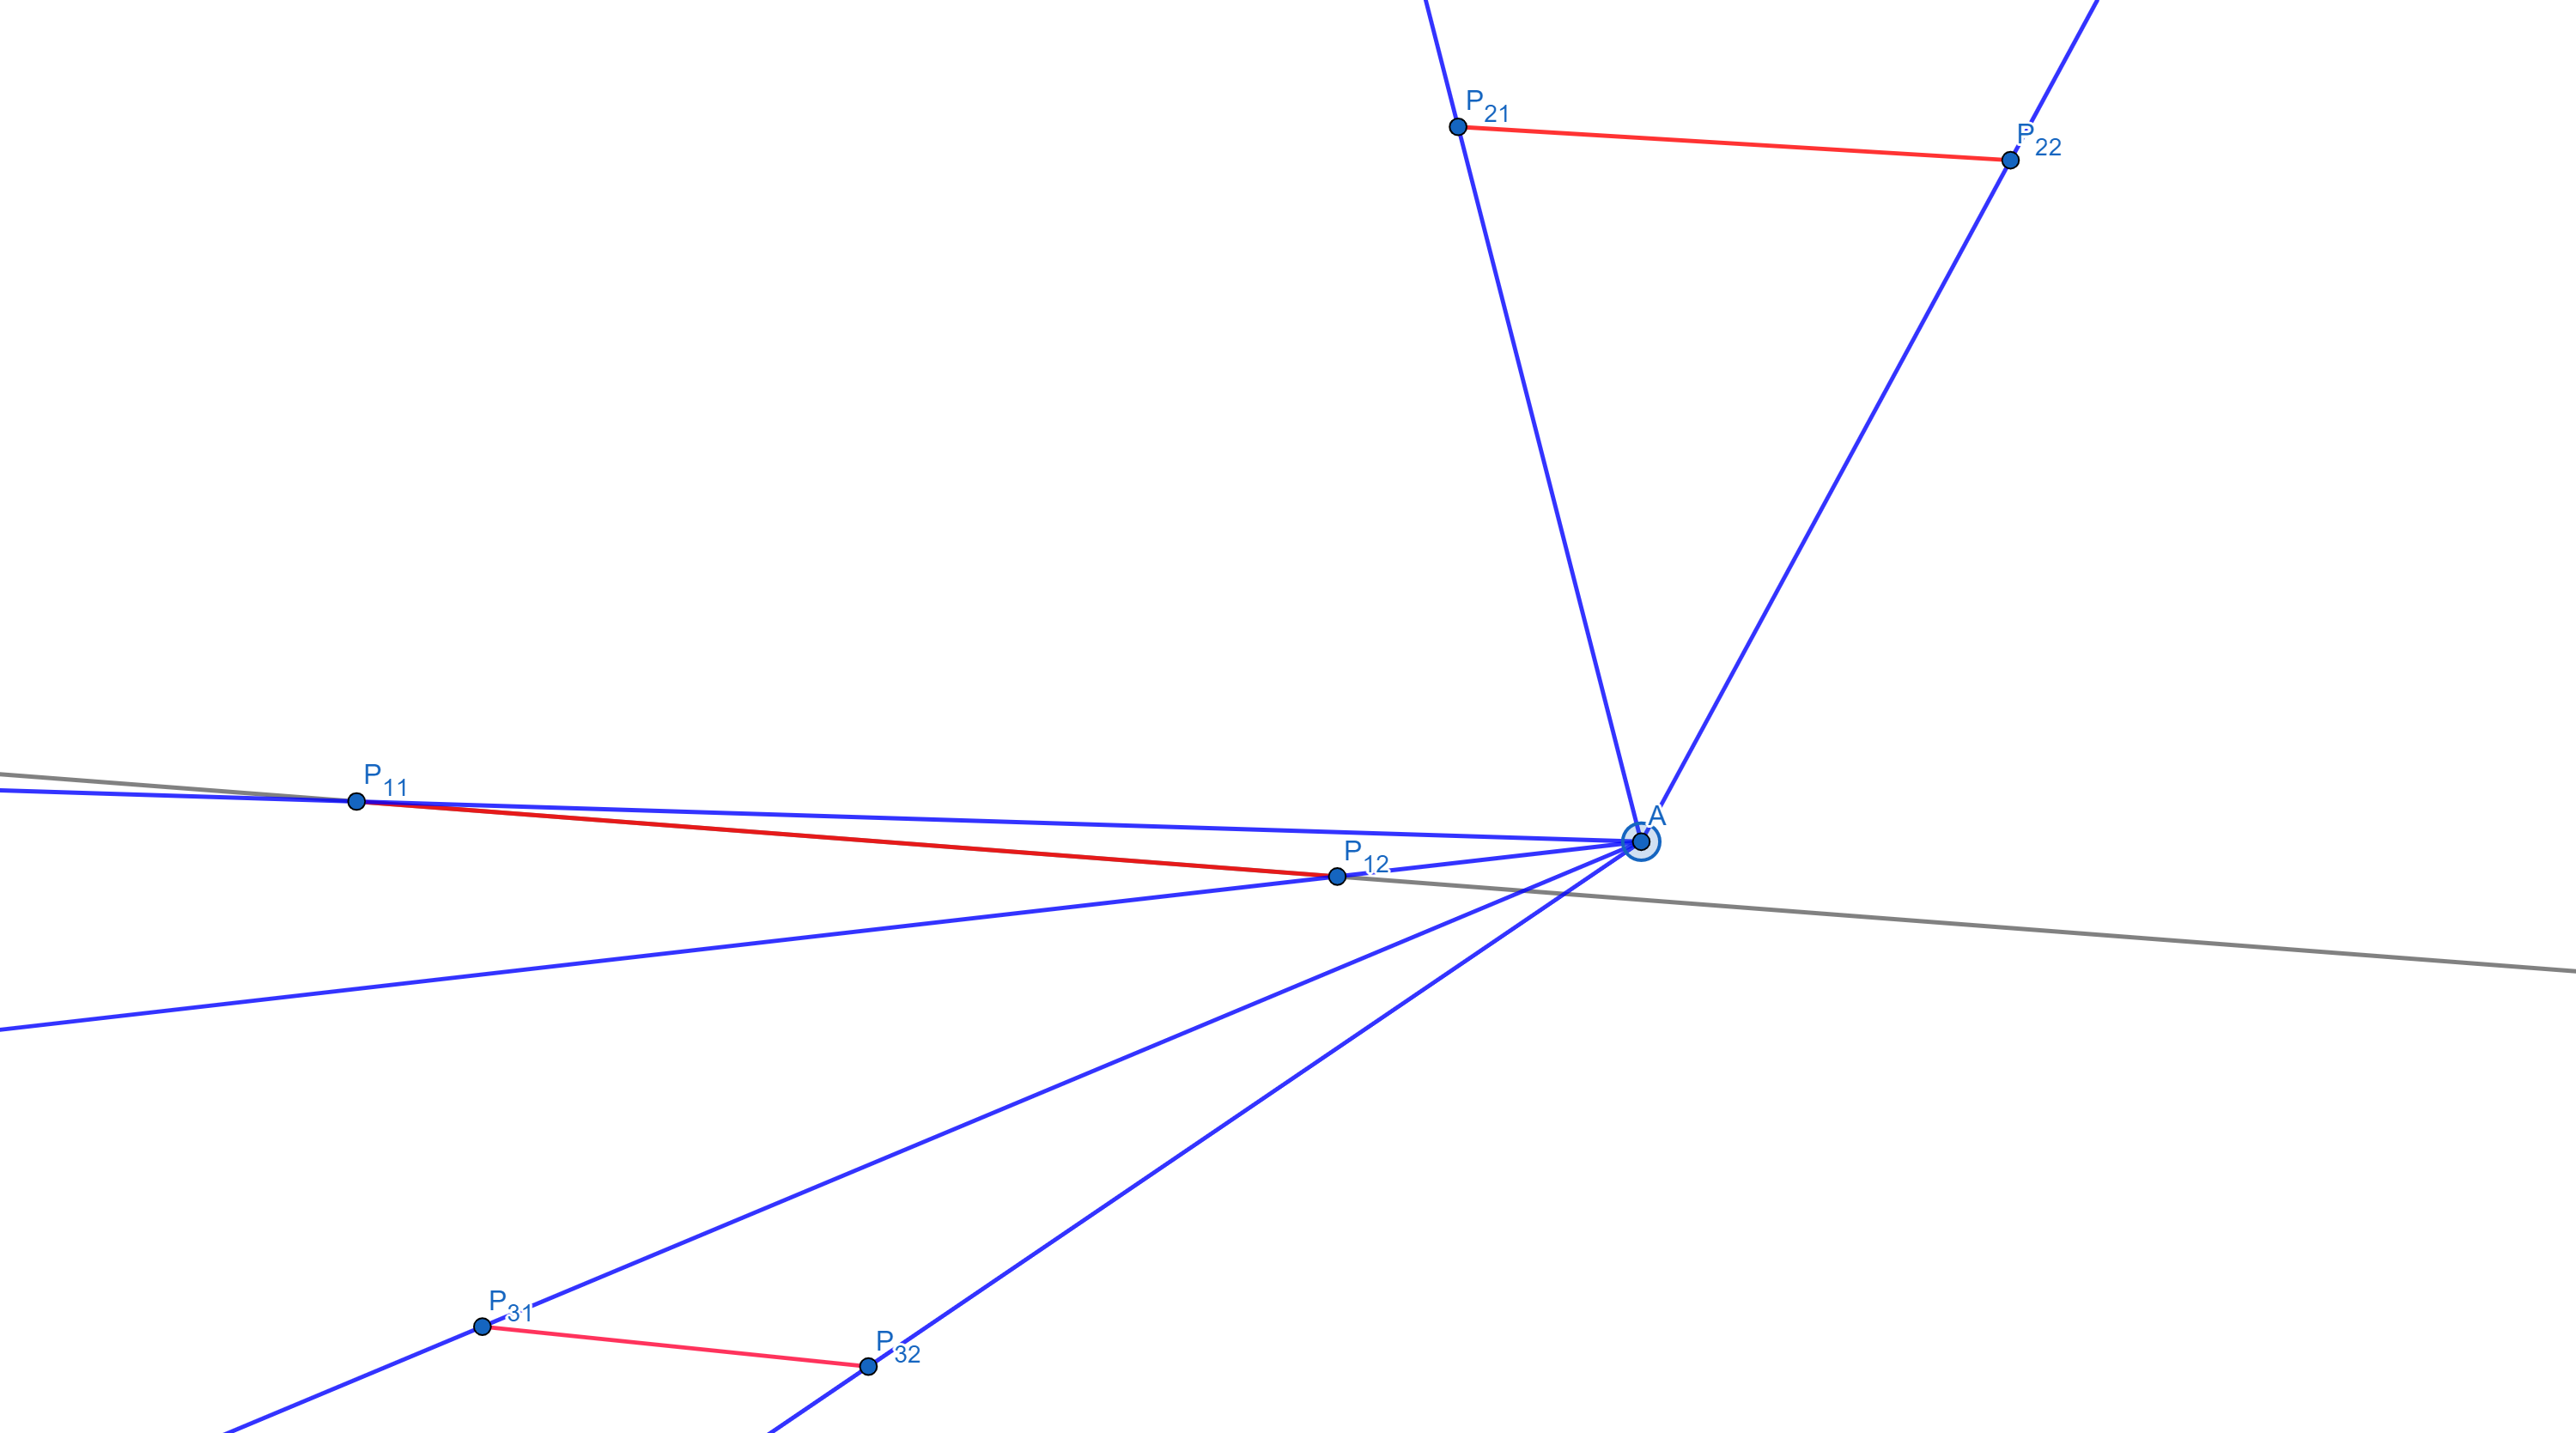
\includegraphics[width=0.5\linewidth]{near_segment_1.png}
            \end{figure}
            \begin{figure}[h]
            \centering
            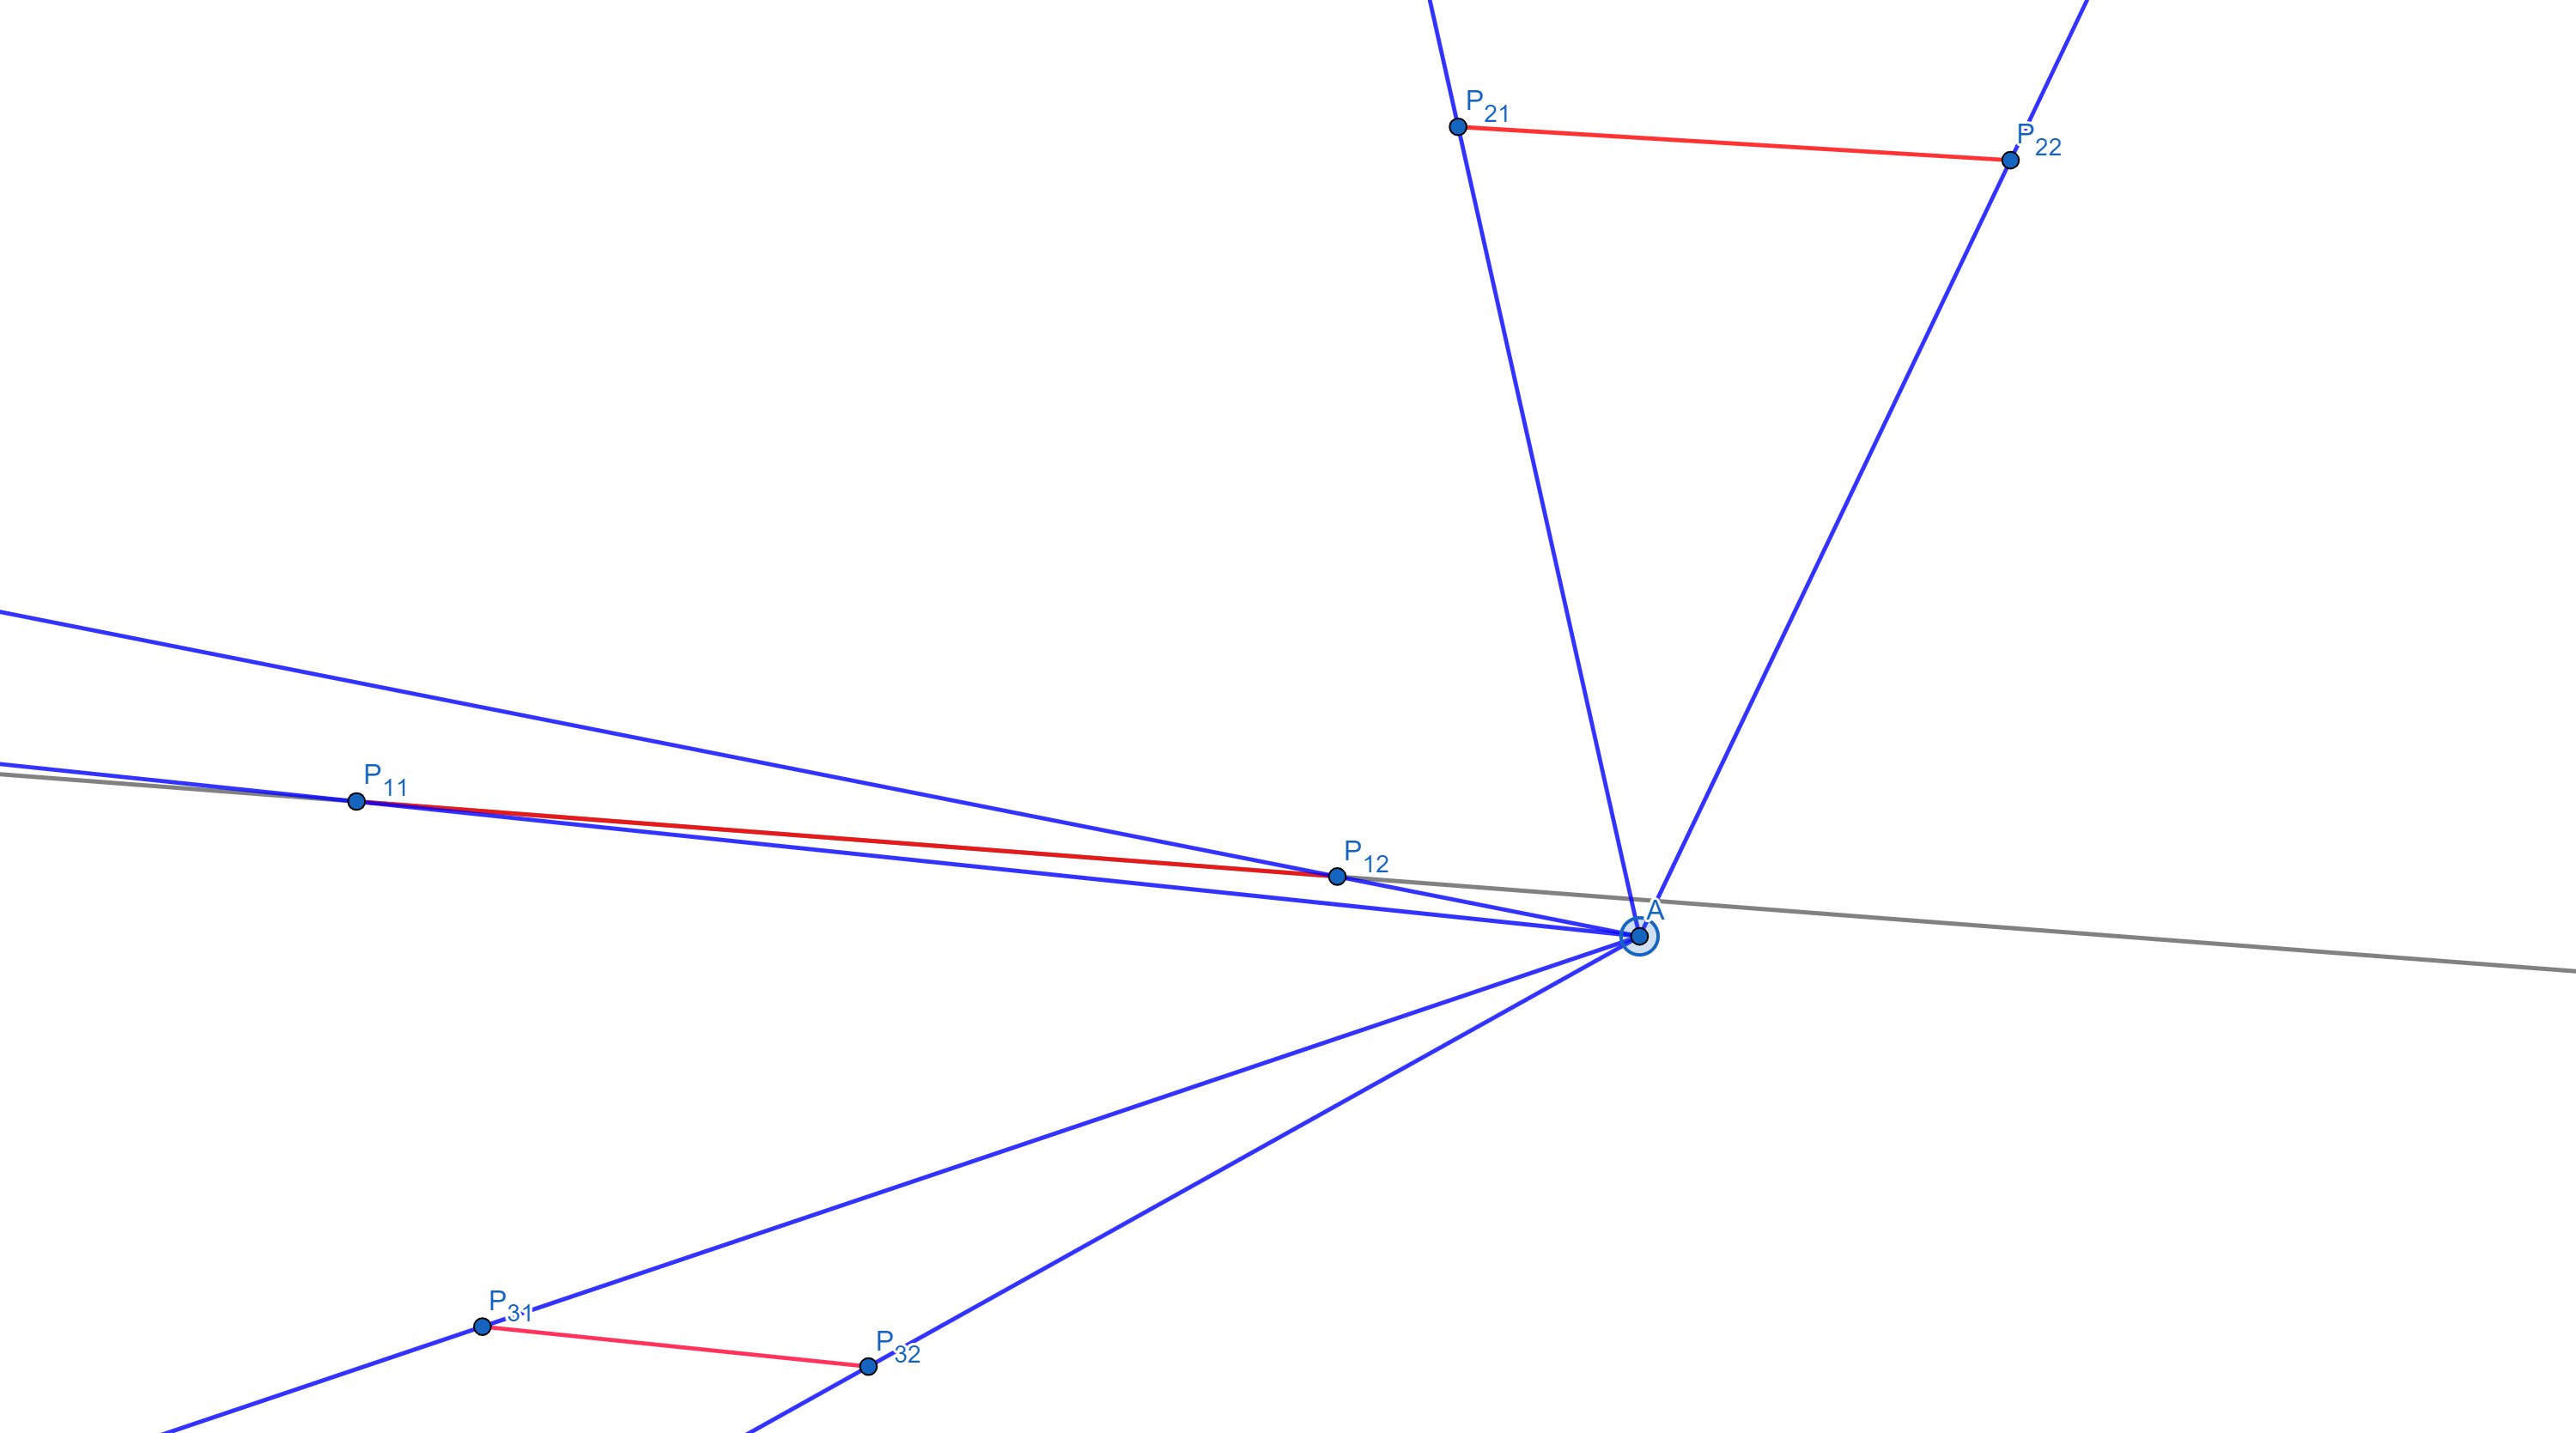
\includegraphics[width=0.5\linewidth]{near_segment_2.png}
            \end{figure}
      \item Необходимо честно пересчитать <<правильность>> отрезка
            с выбором точки внутри грани. %нет?
            \begin{figure}[H]
            \centering
            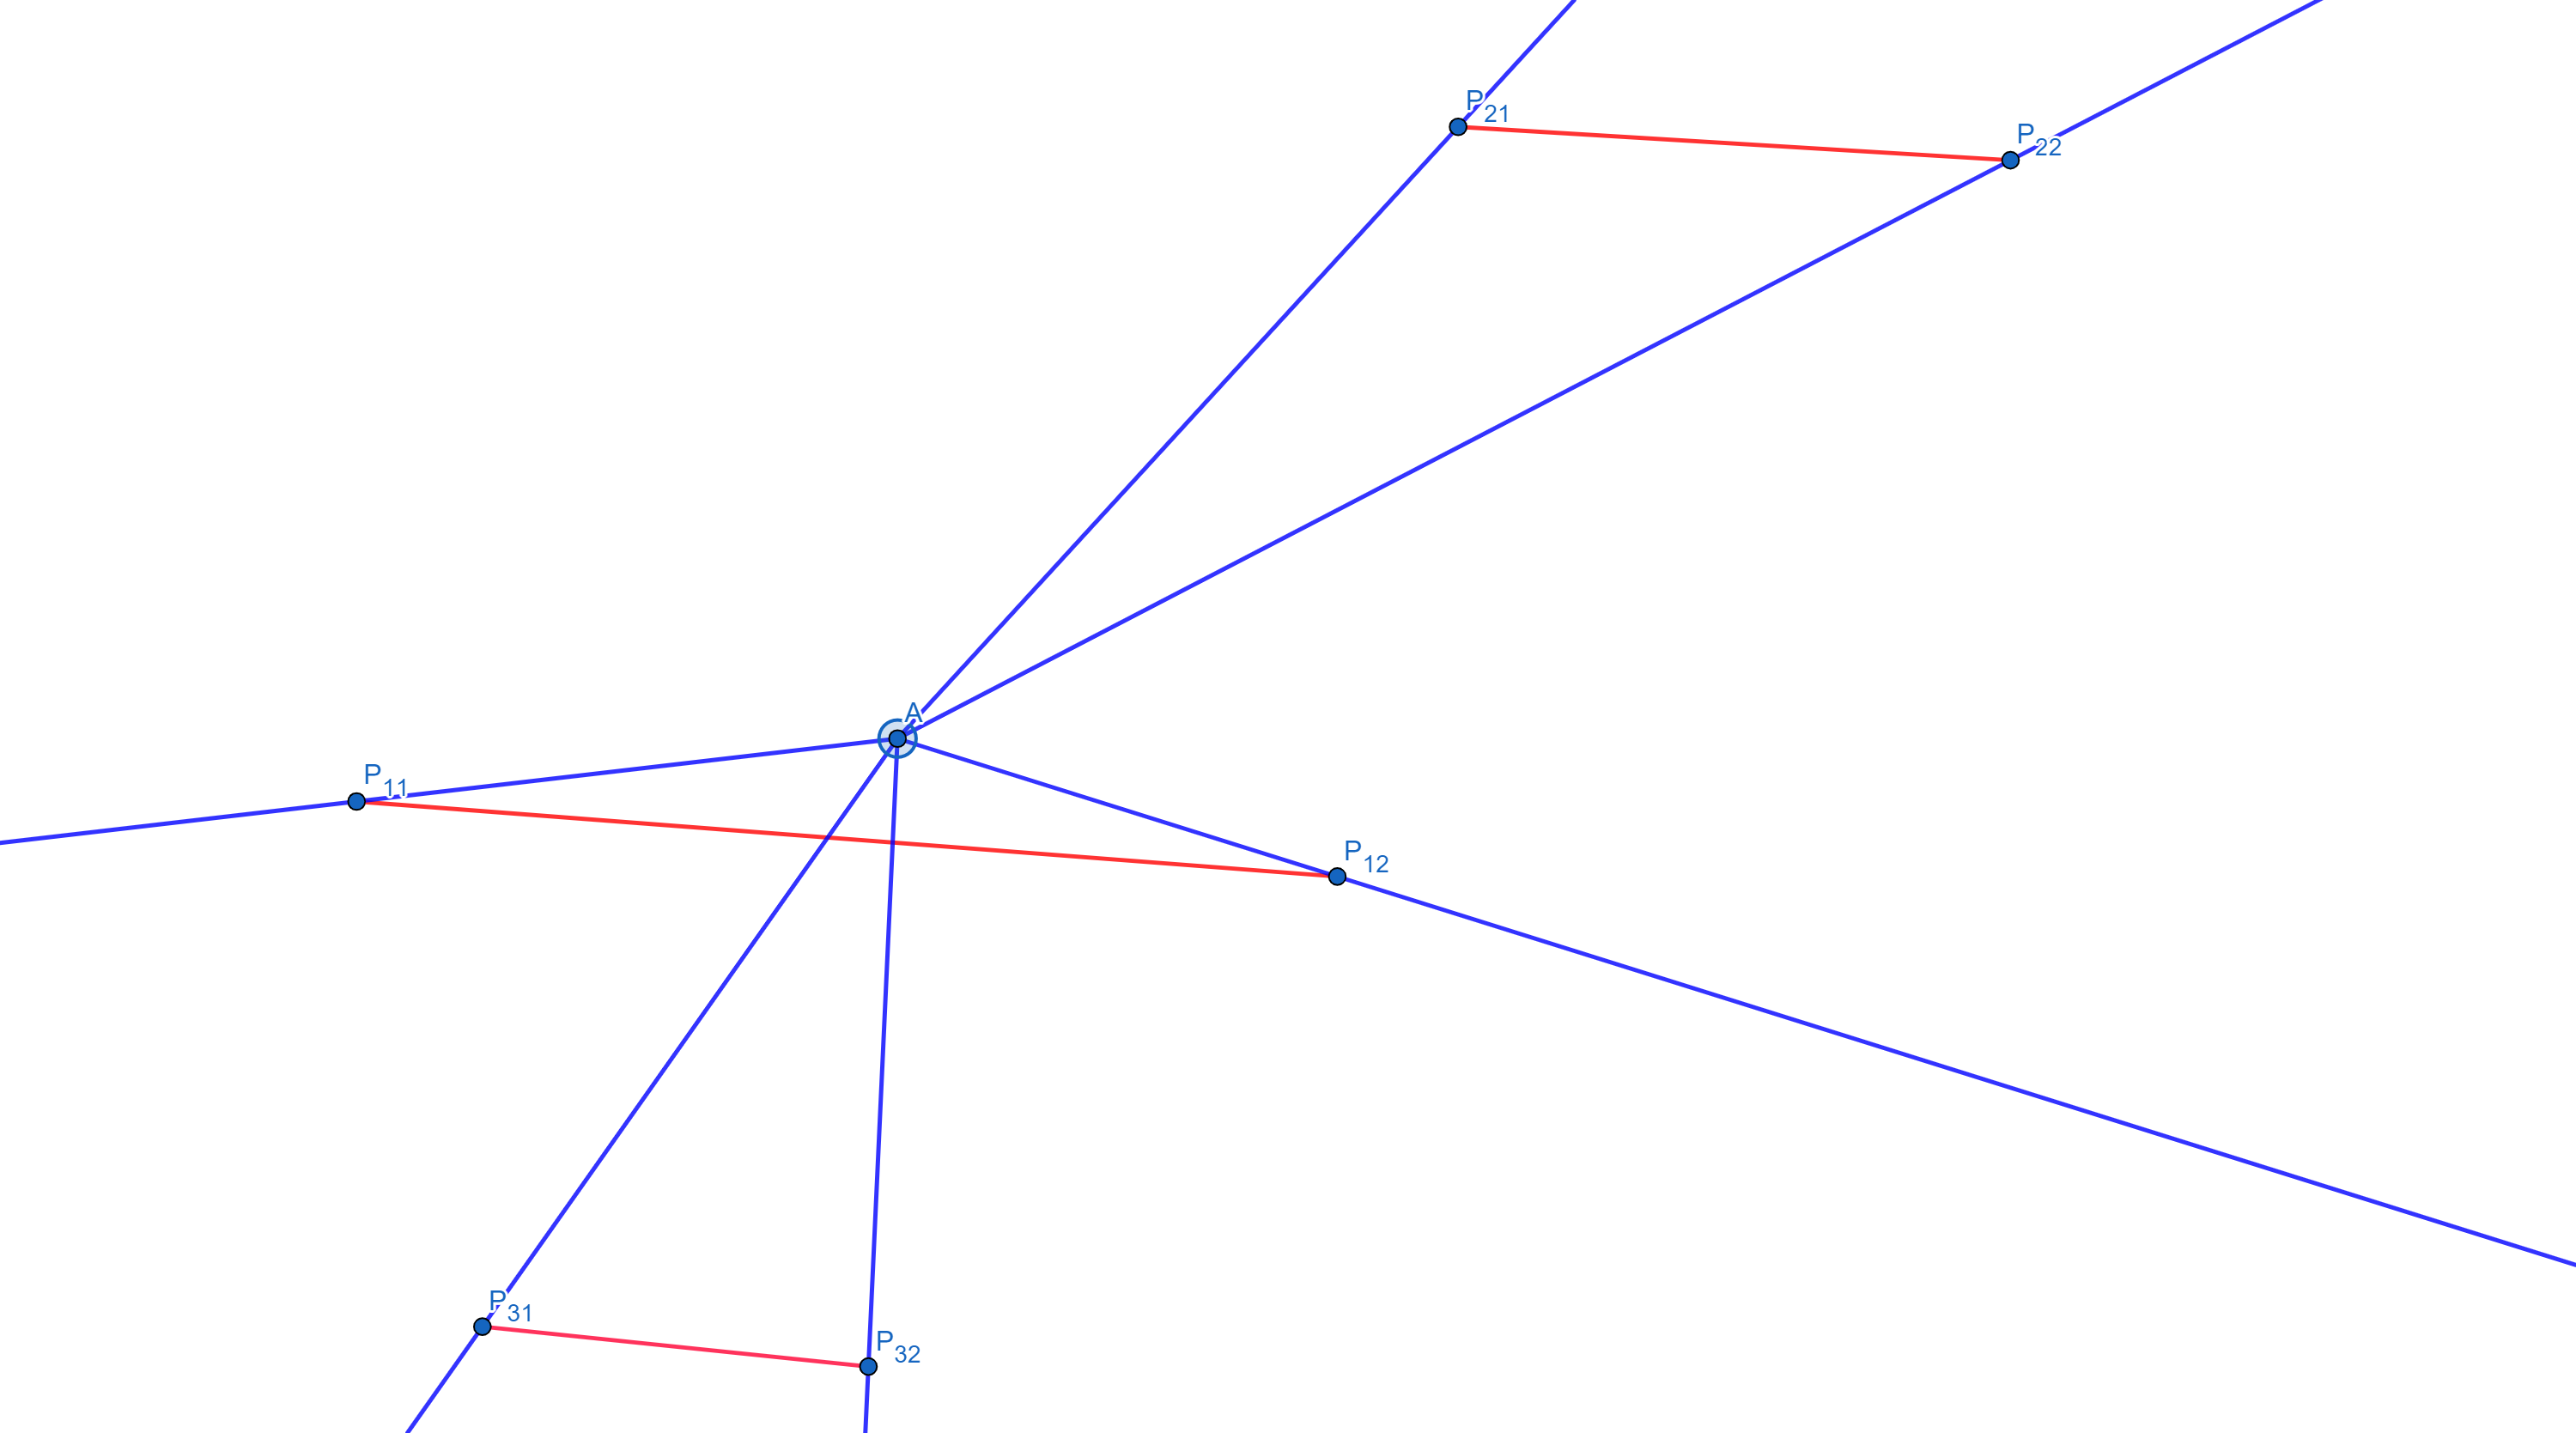
\includegraphics[width=0.5\linewidth]{segment_1.png}
            \end{figure}
            \begin{figure}[H]
            \centering
            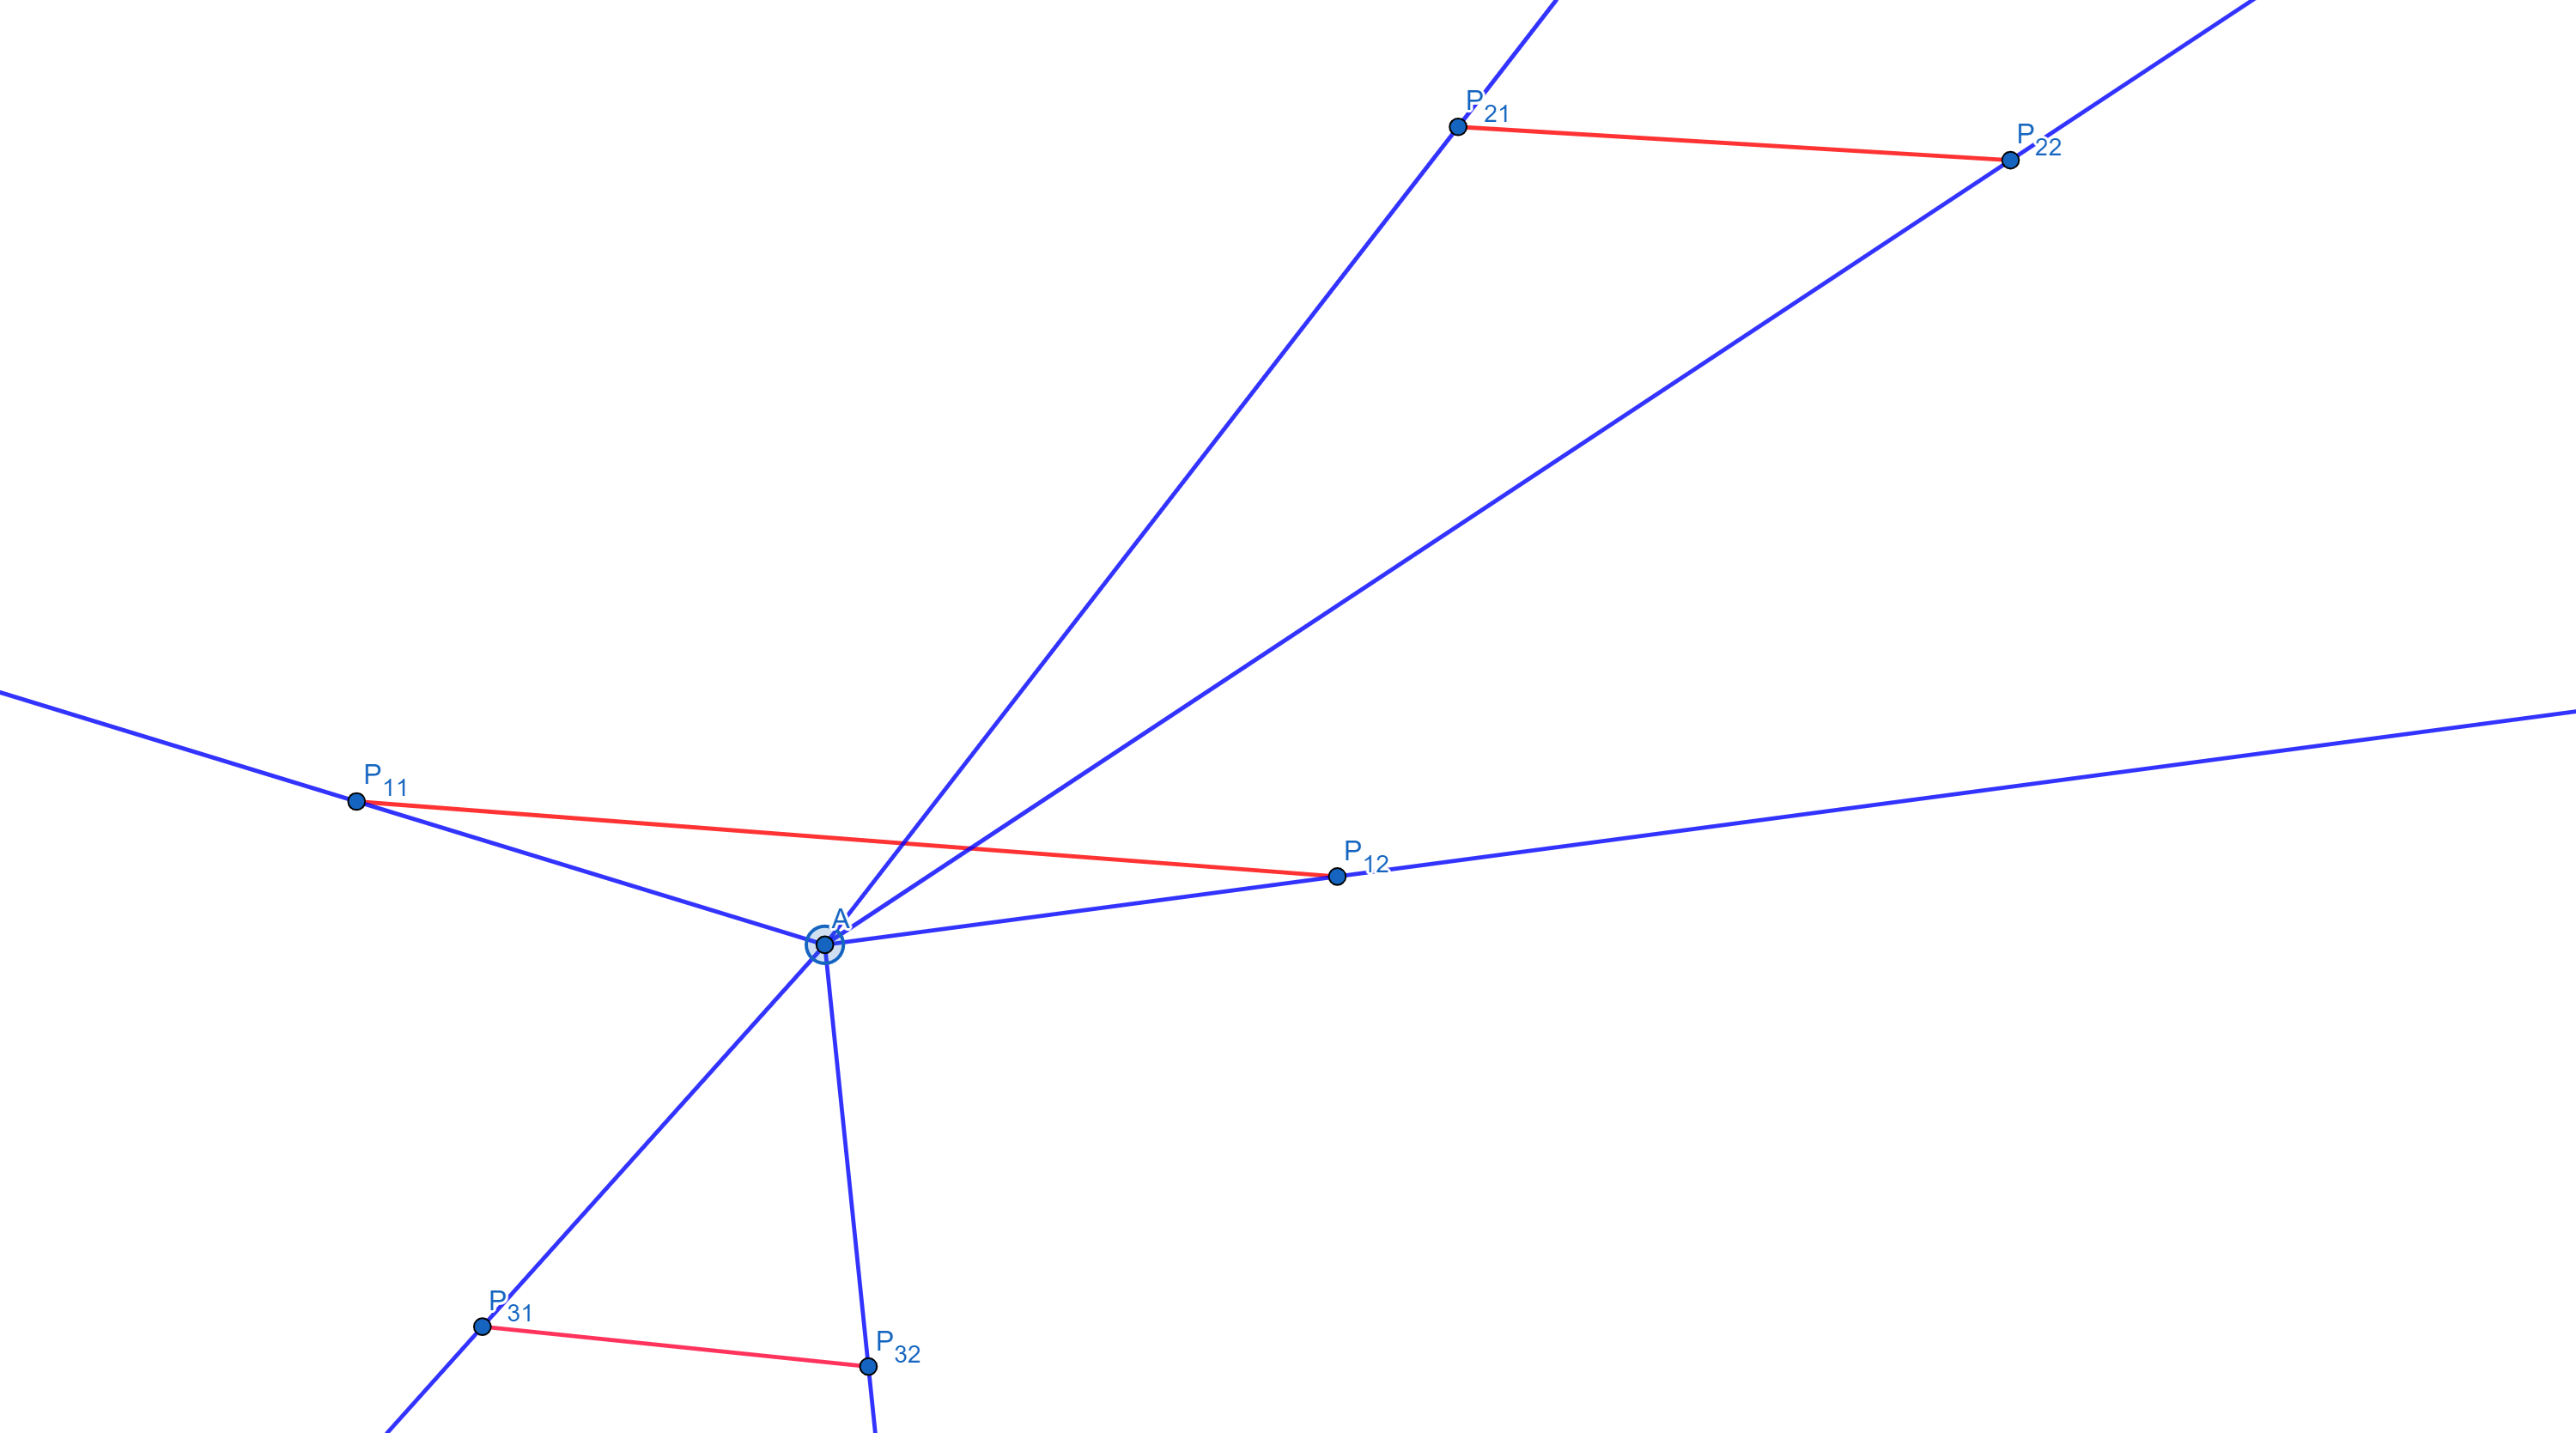
\includegraphics[width=0.5\linewidth]{segment_2.png}
            \end{figure}
      \item Точки $p_i, p_j$ меняются местами в массиве. <<Правильность>>
            обоих отрезков при прямом переходе (от первого рисунка ко второму)
            необходимо пересчитывать честно с выбором точки внутри грани, %нет?
            при обратном переходе оба отрезка перестают быть <<правильными>>
            (если были).
            \begin{figure}[H]
            \centering
            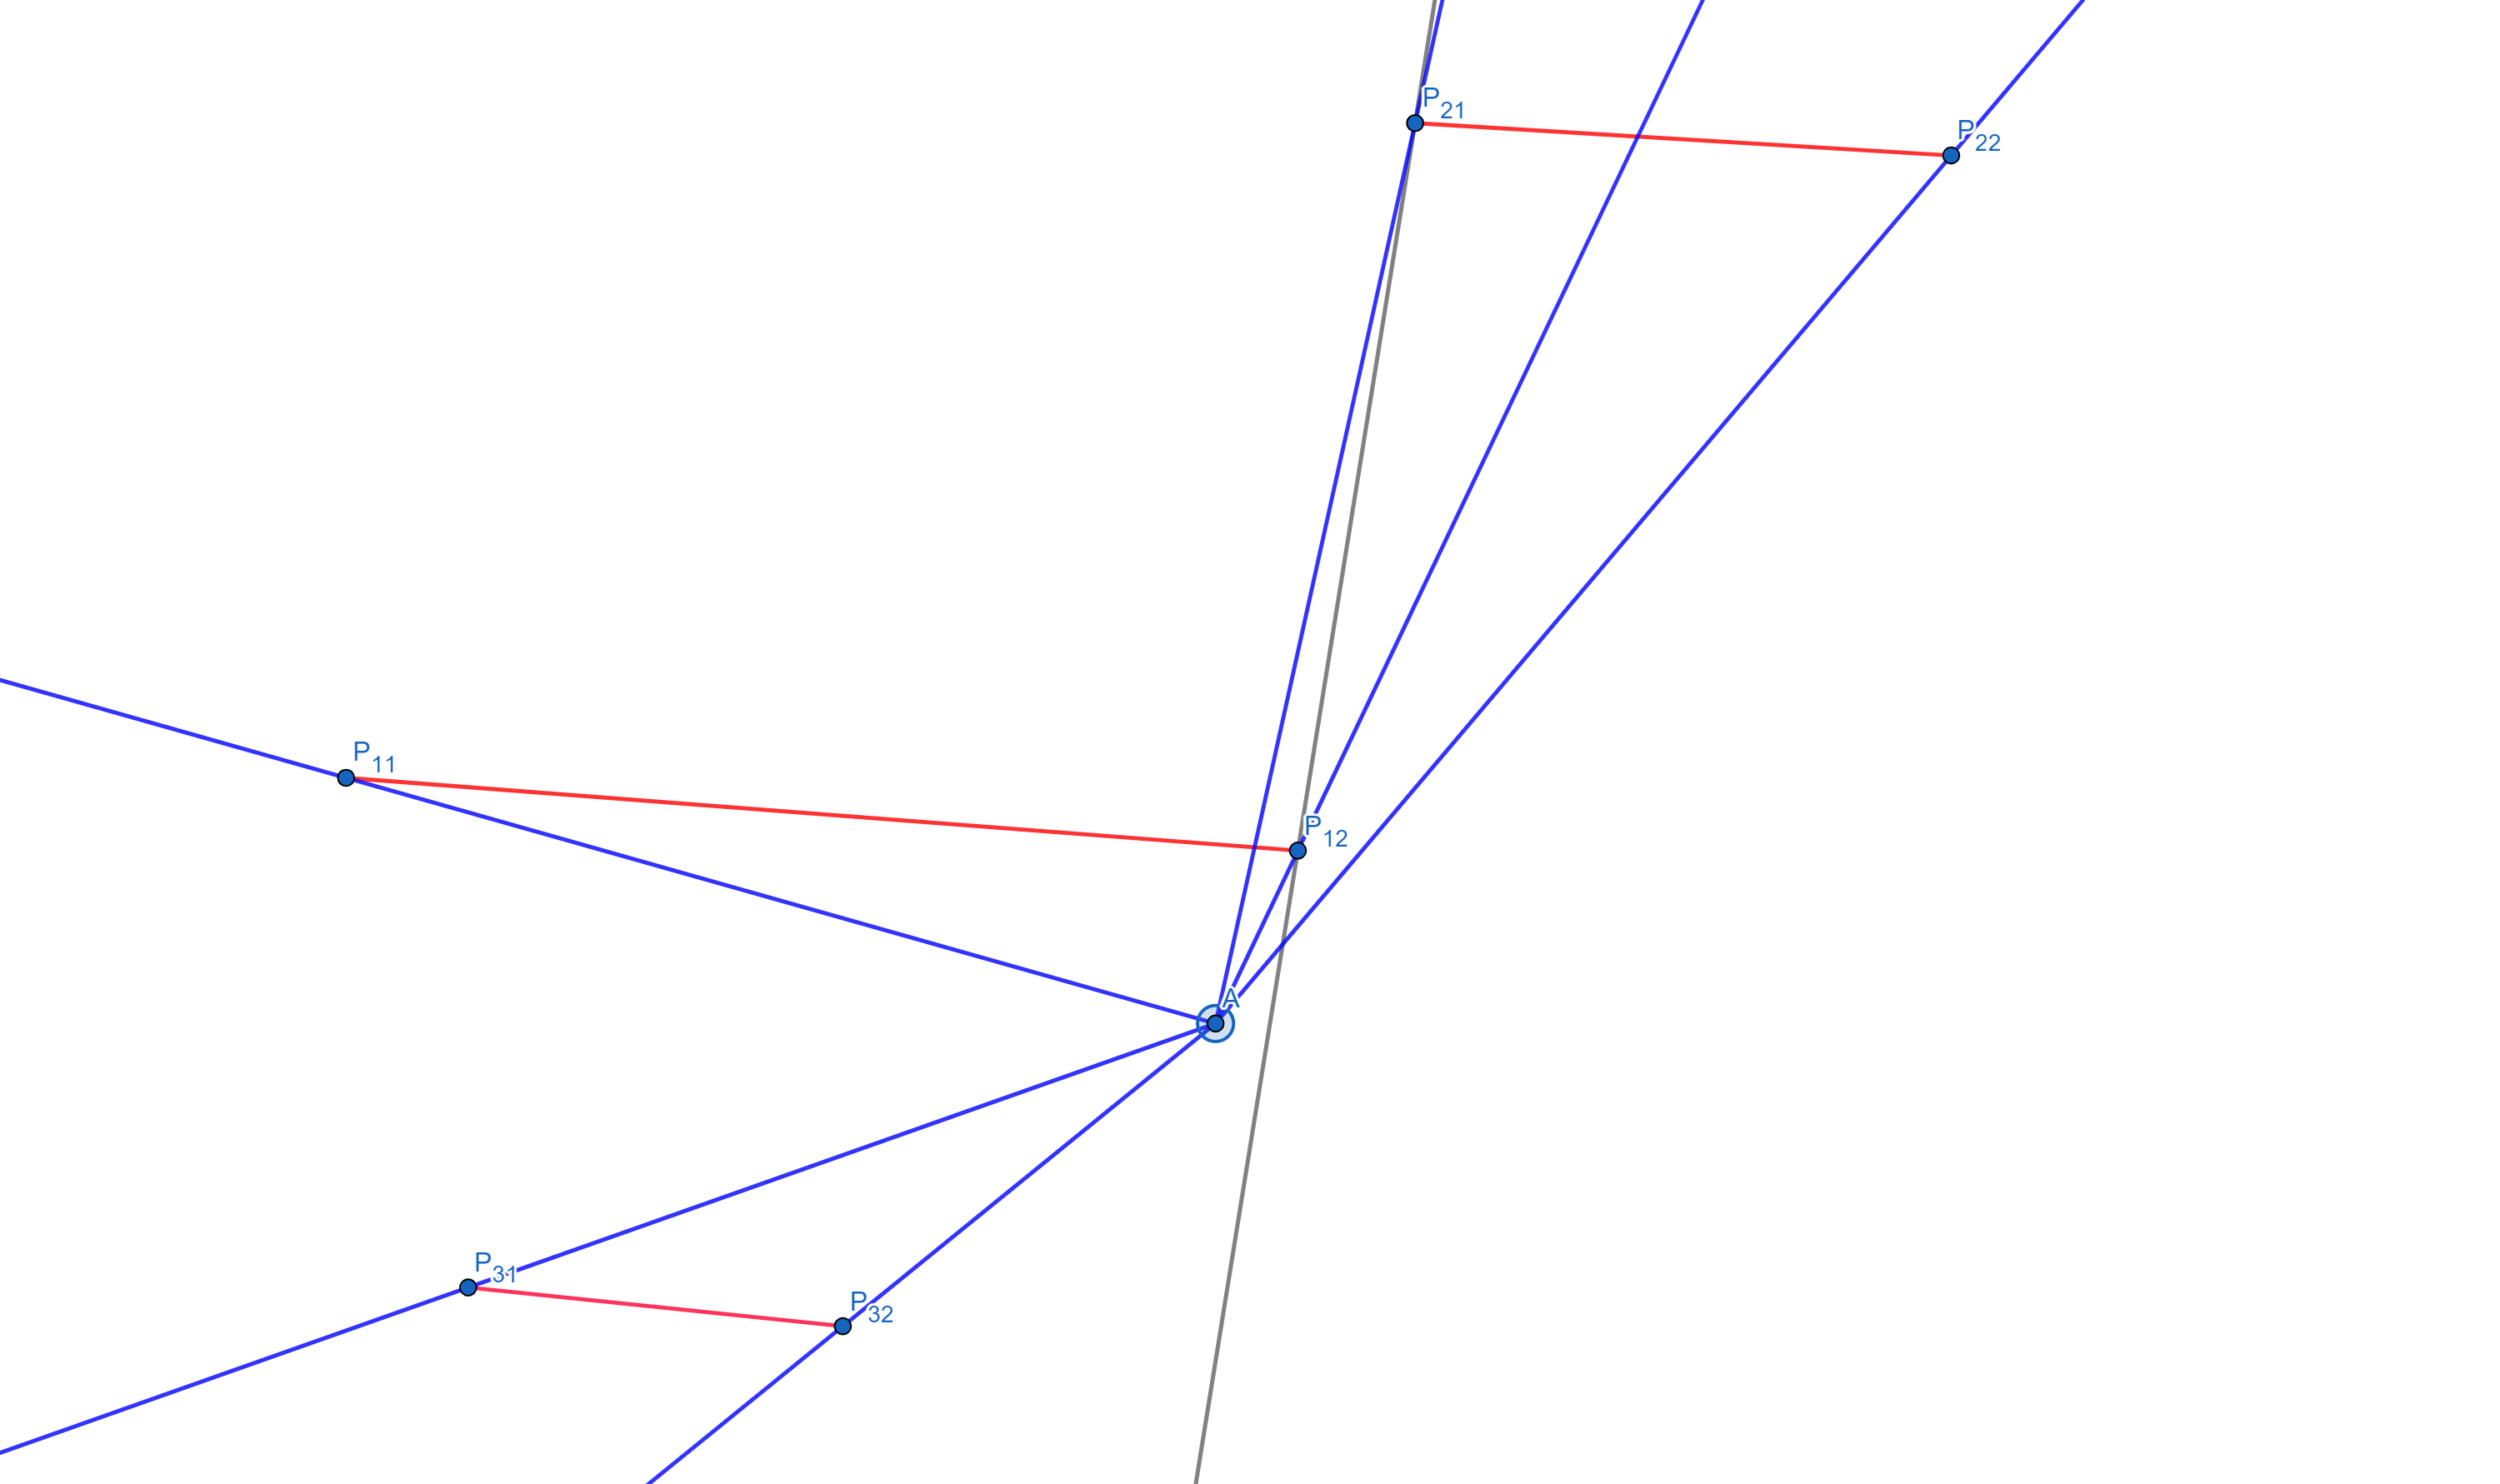
\includegraphics[width=0.5\linewidth]{one_side_1_1.png}
            \end{figure}
            \begin{figure}[H]
            \centering
            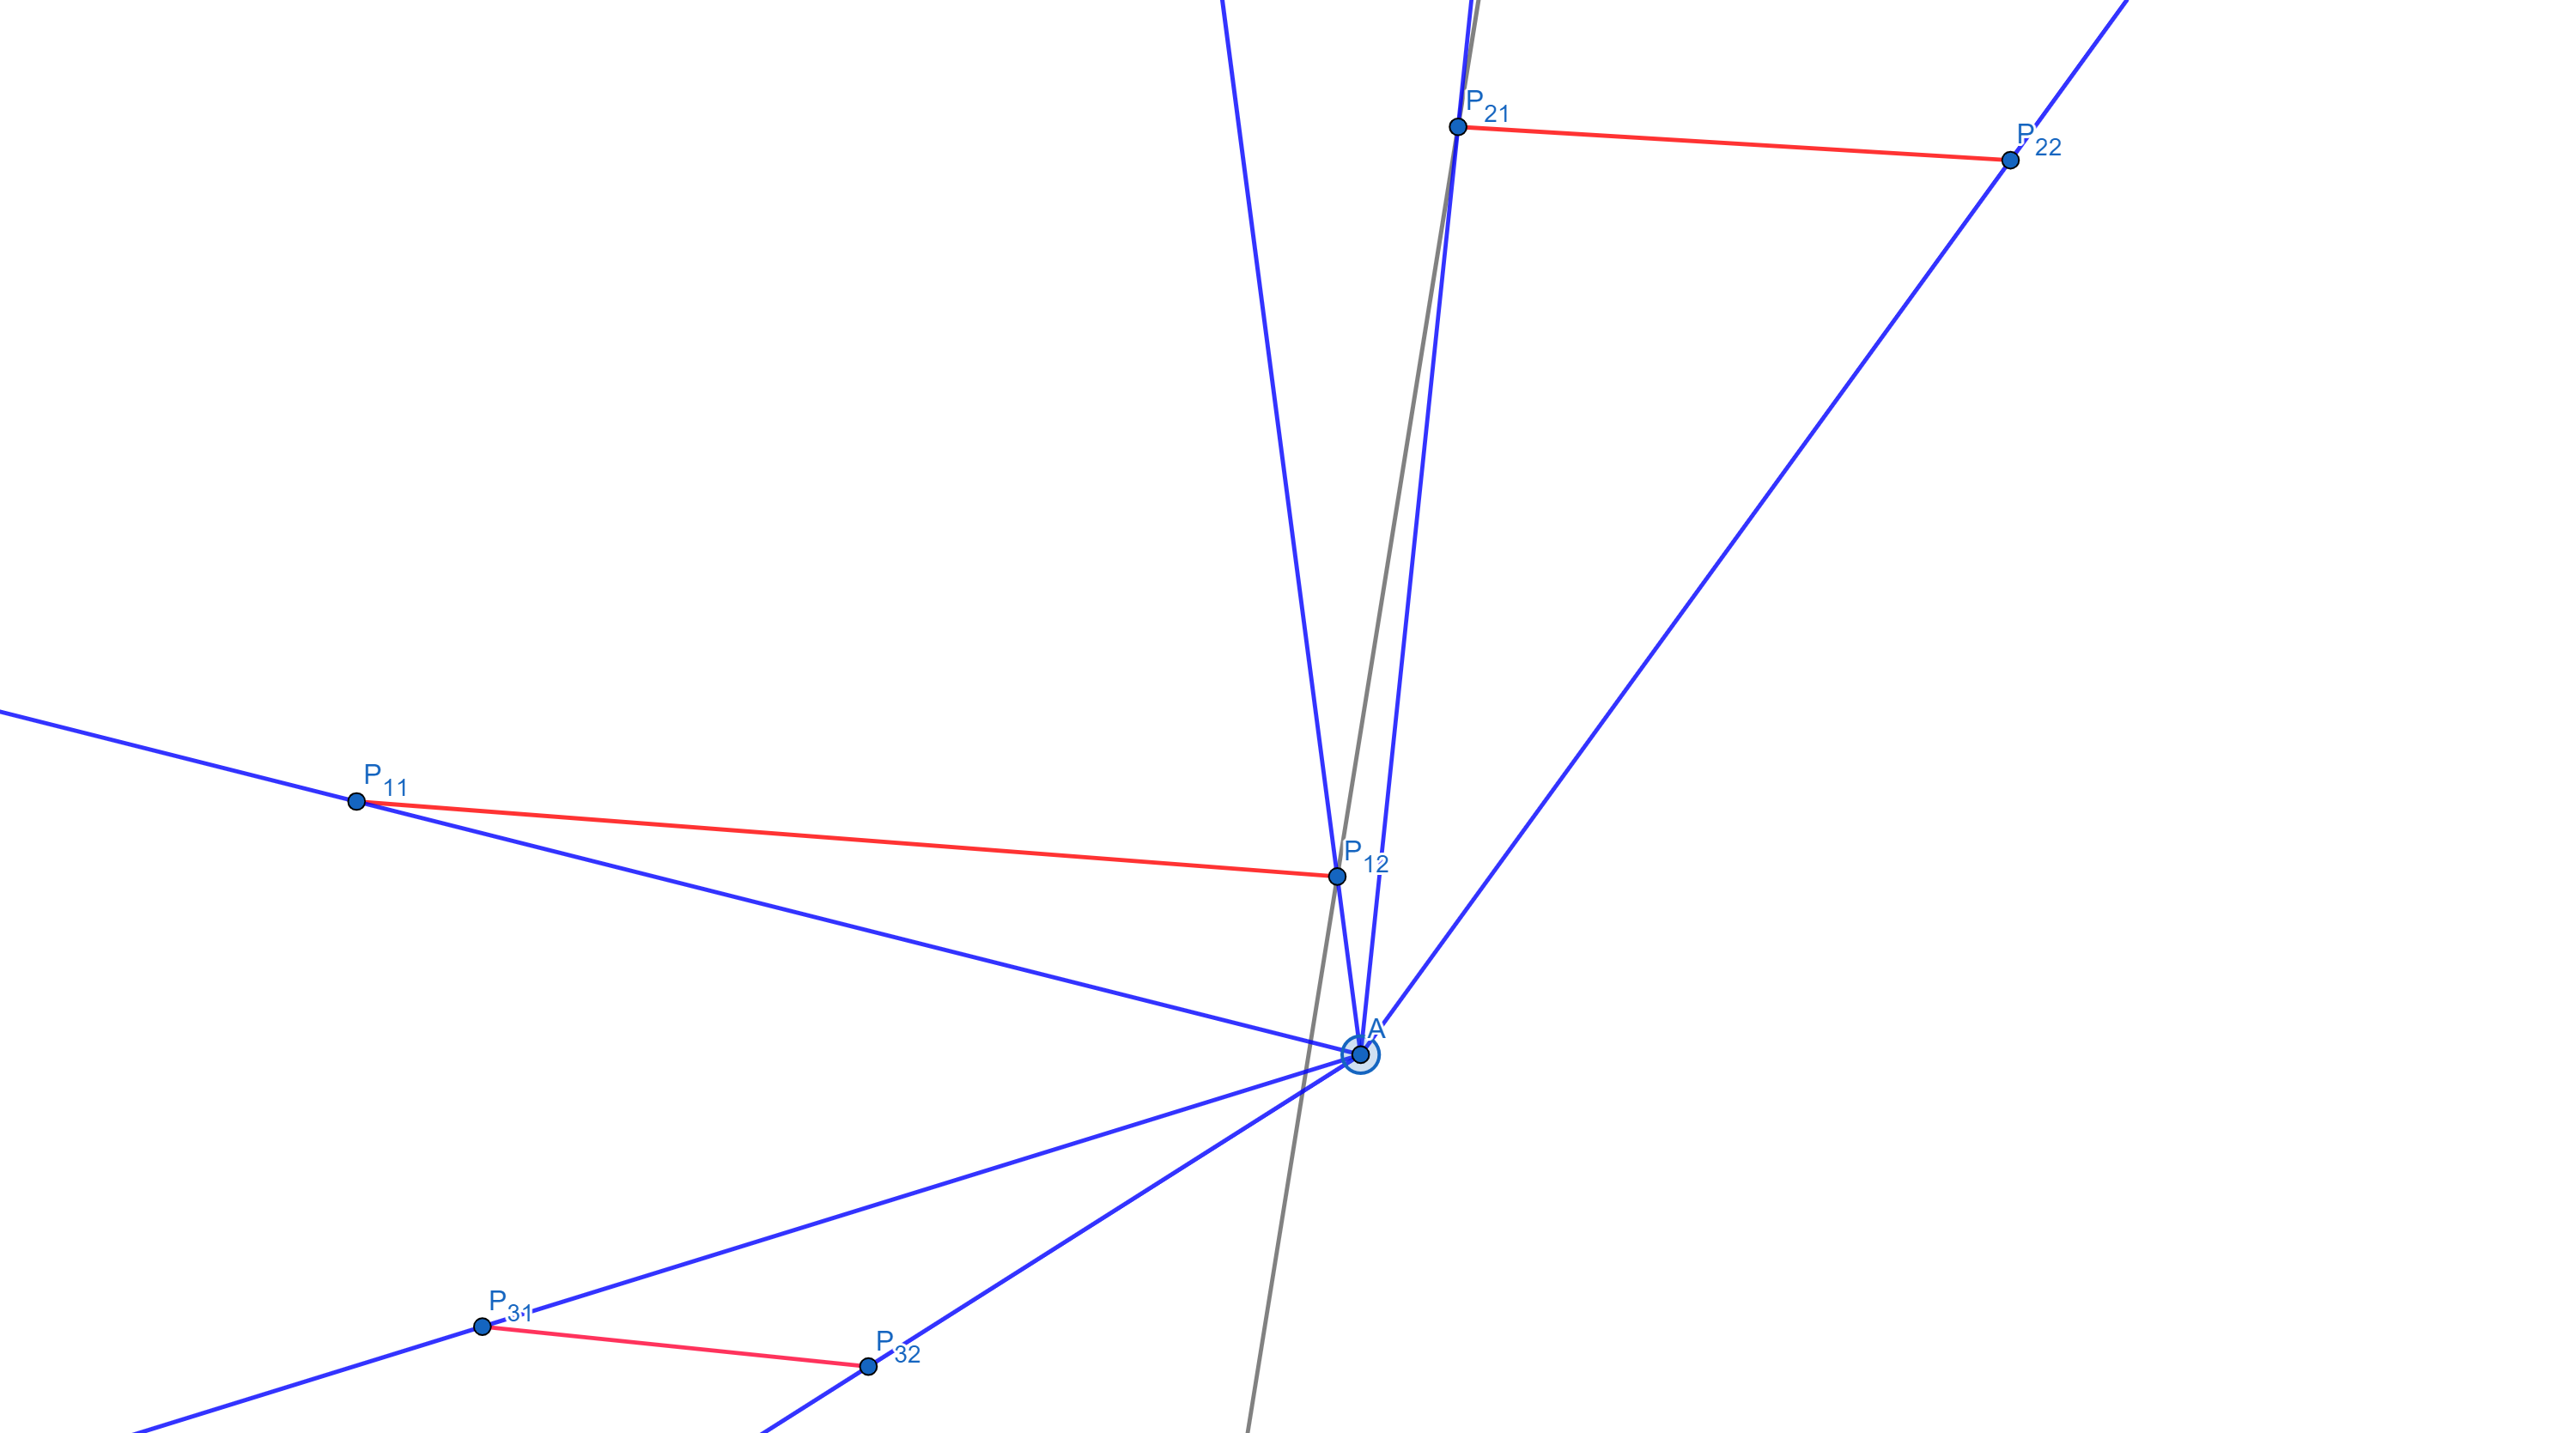
\includegraphics[width=0.5\linewidth]{one_side_1_2.png}
            \end{figure}
      \item Точки $p_i, p_j$ меняются местами в массиве, <<правильность>>
            отрезков остается неизменной.
            \begin{figure}[H]
            \centering
            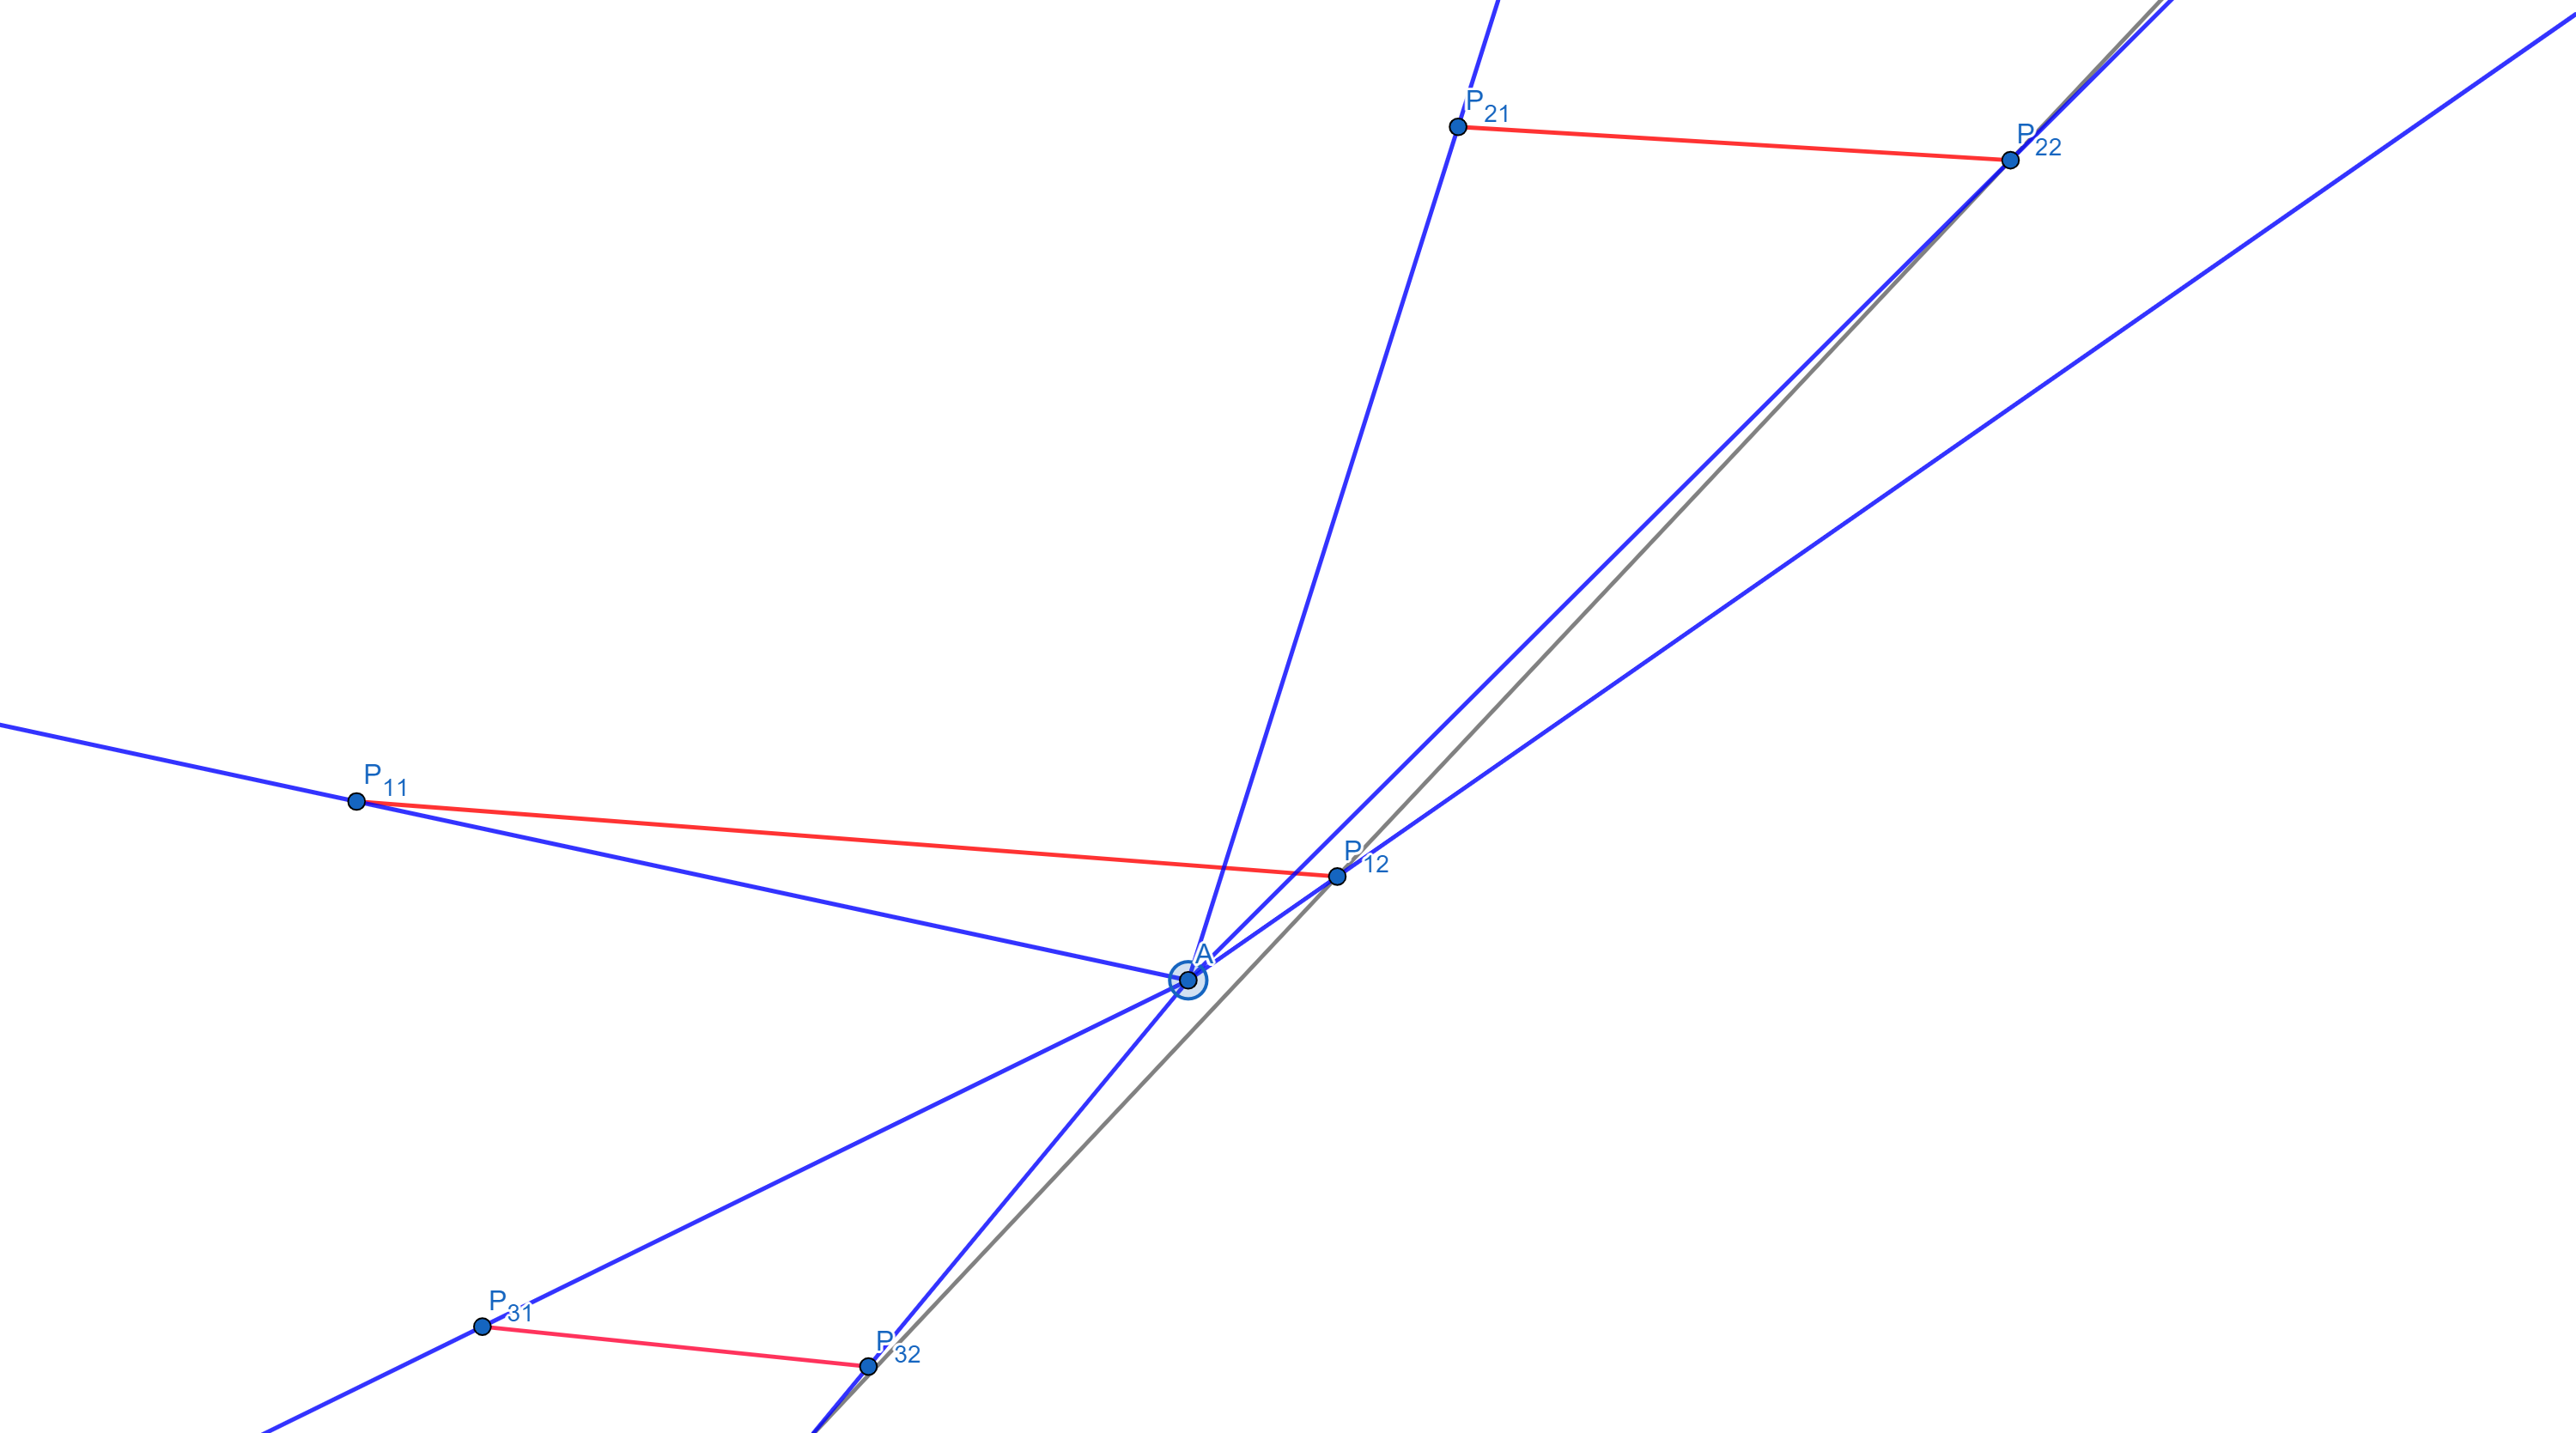
\includegraphics[width=0.5\linewidth]{one_side_2_1.png}
            \end{figure}
            \begin{figure}[H]
            \centering
            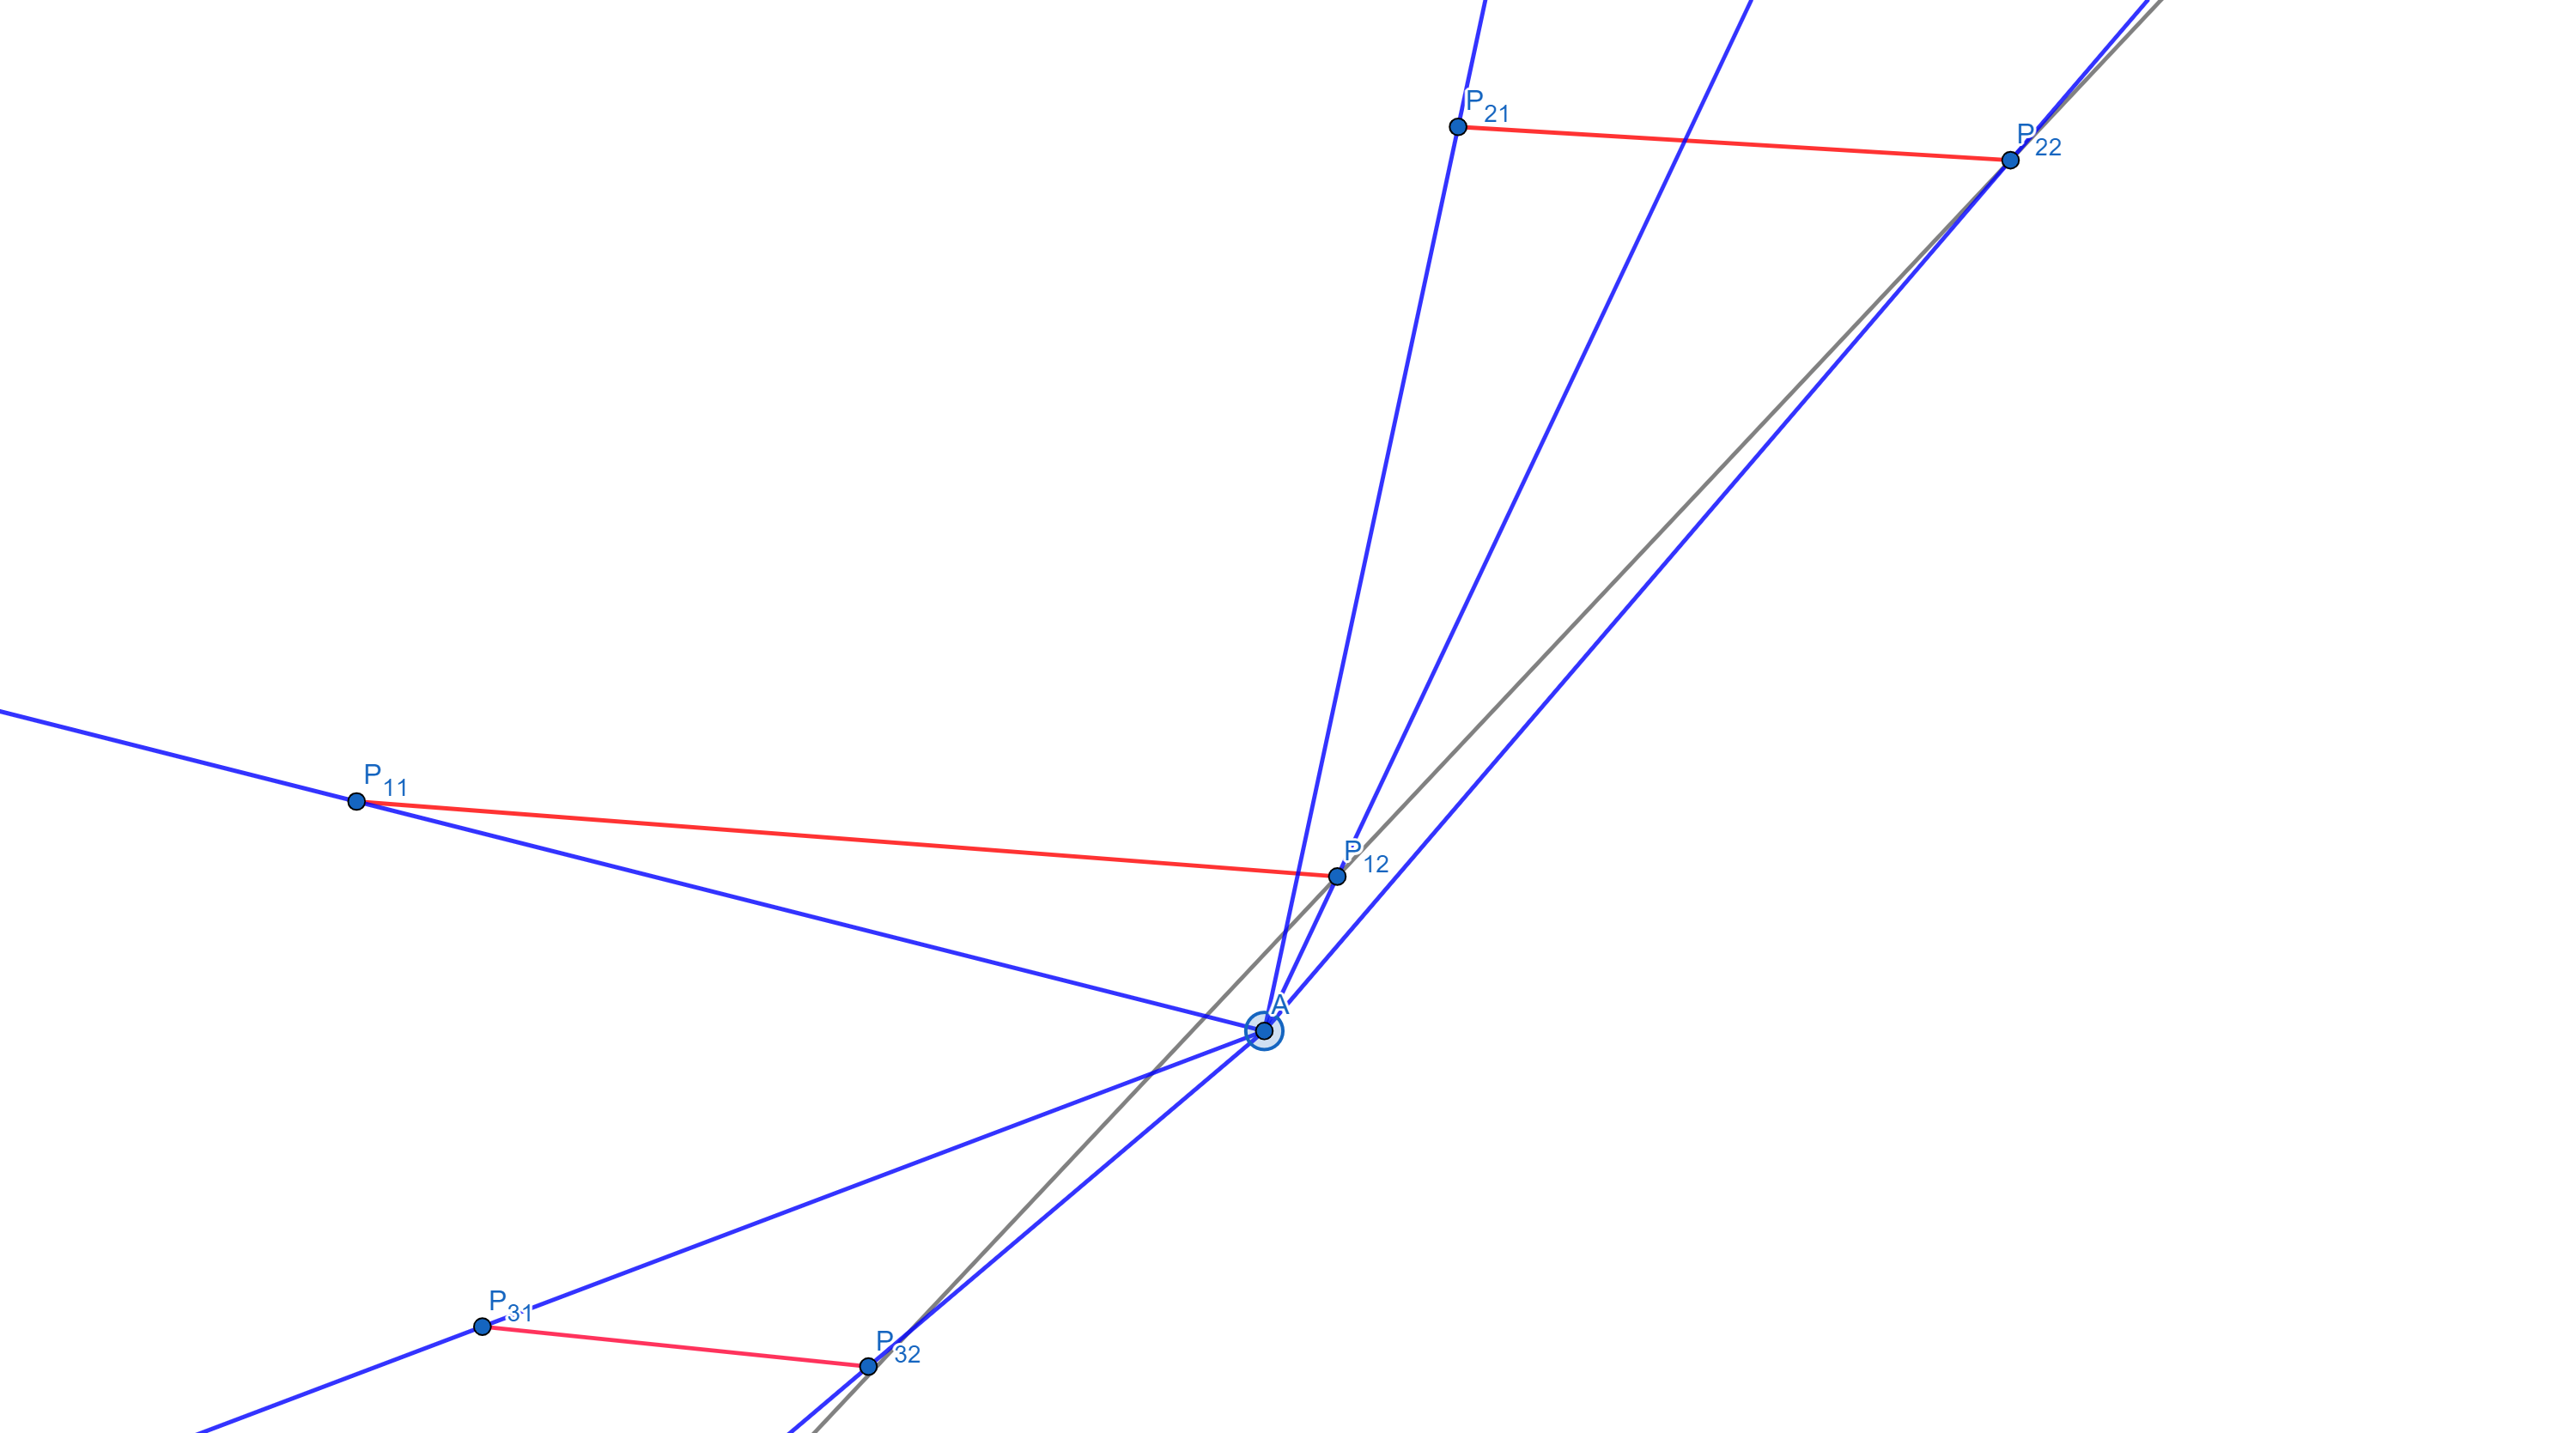
\includegraphics[width=0.5\linewidth]{one_side_2_2.png}
            \end{figure}
      \item Без изменений.
            \begin{figure}[H]
            \centering
            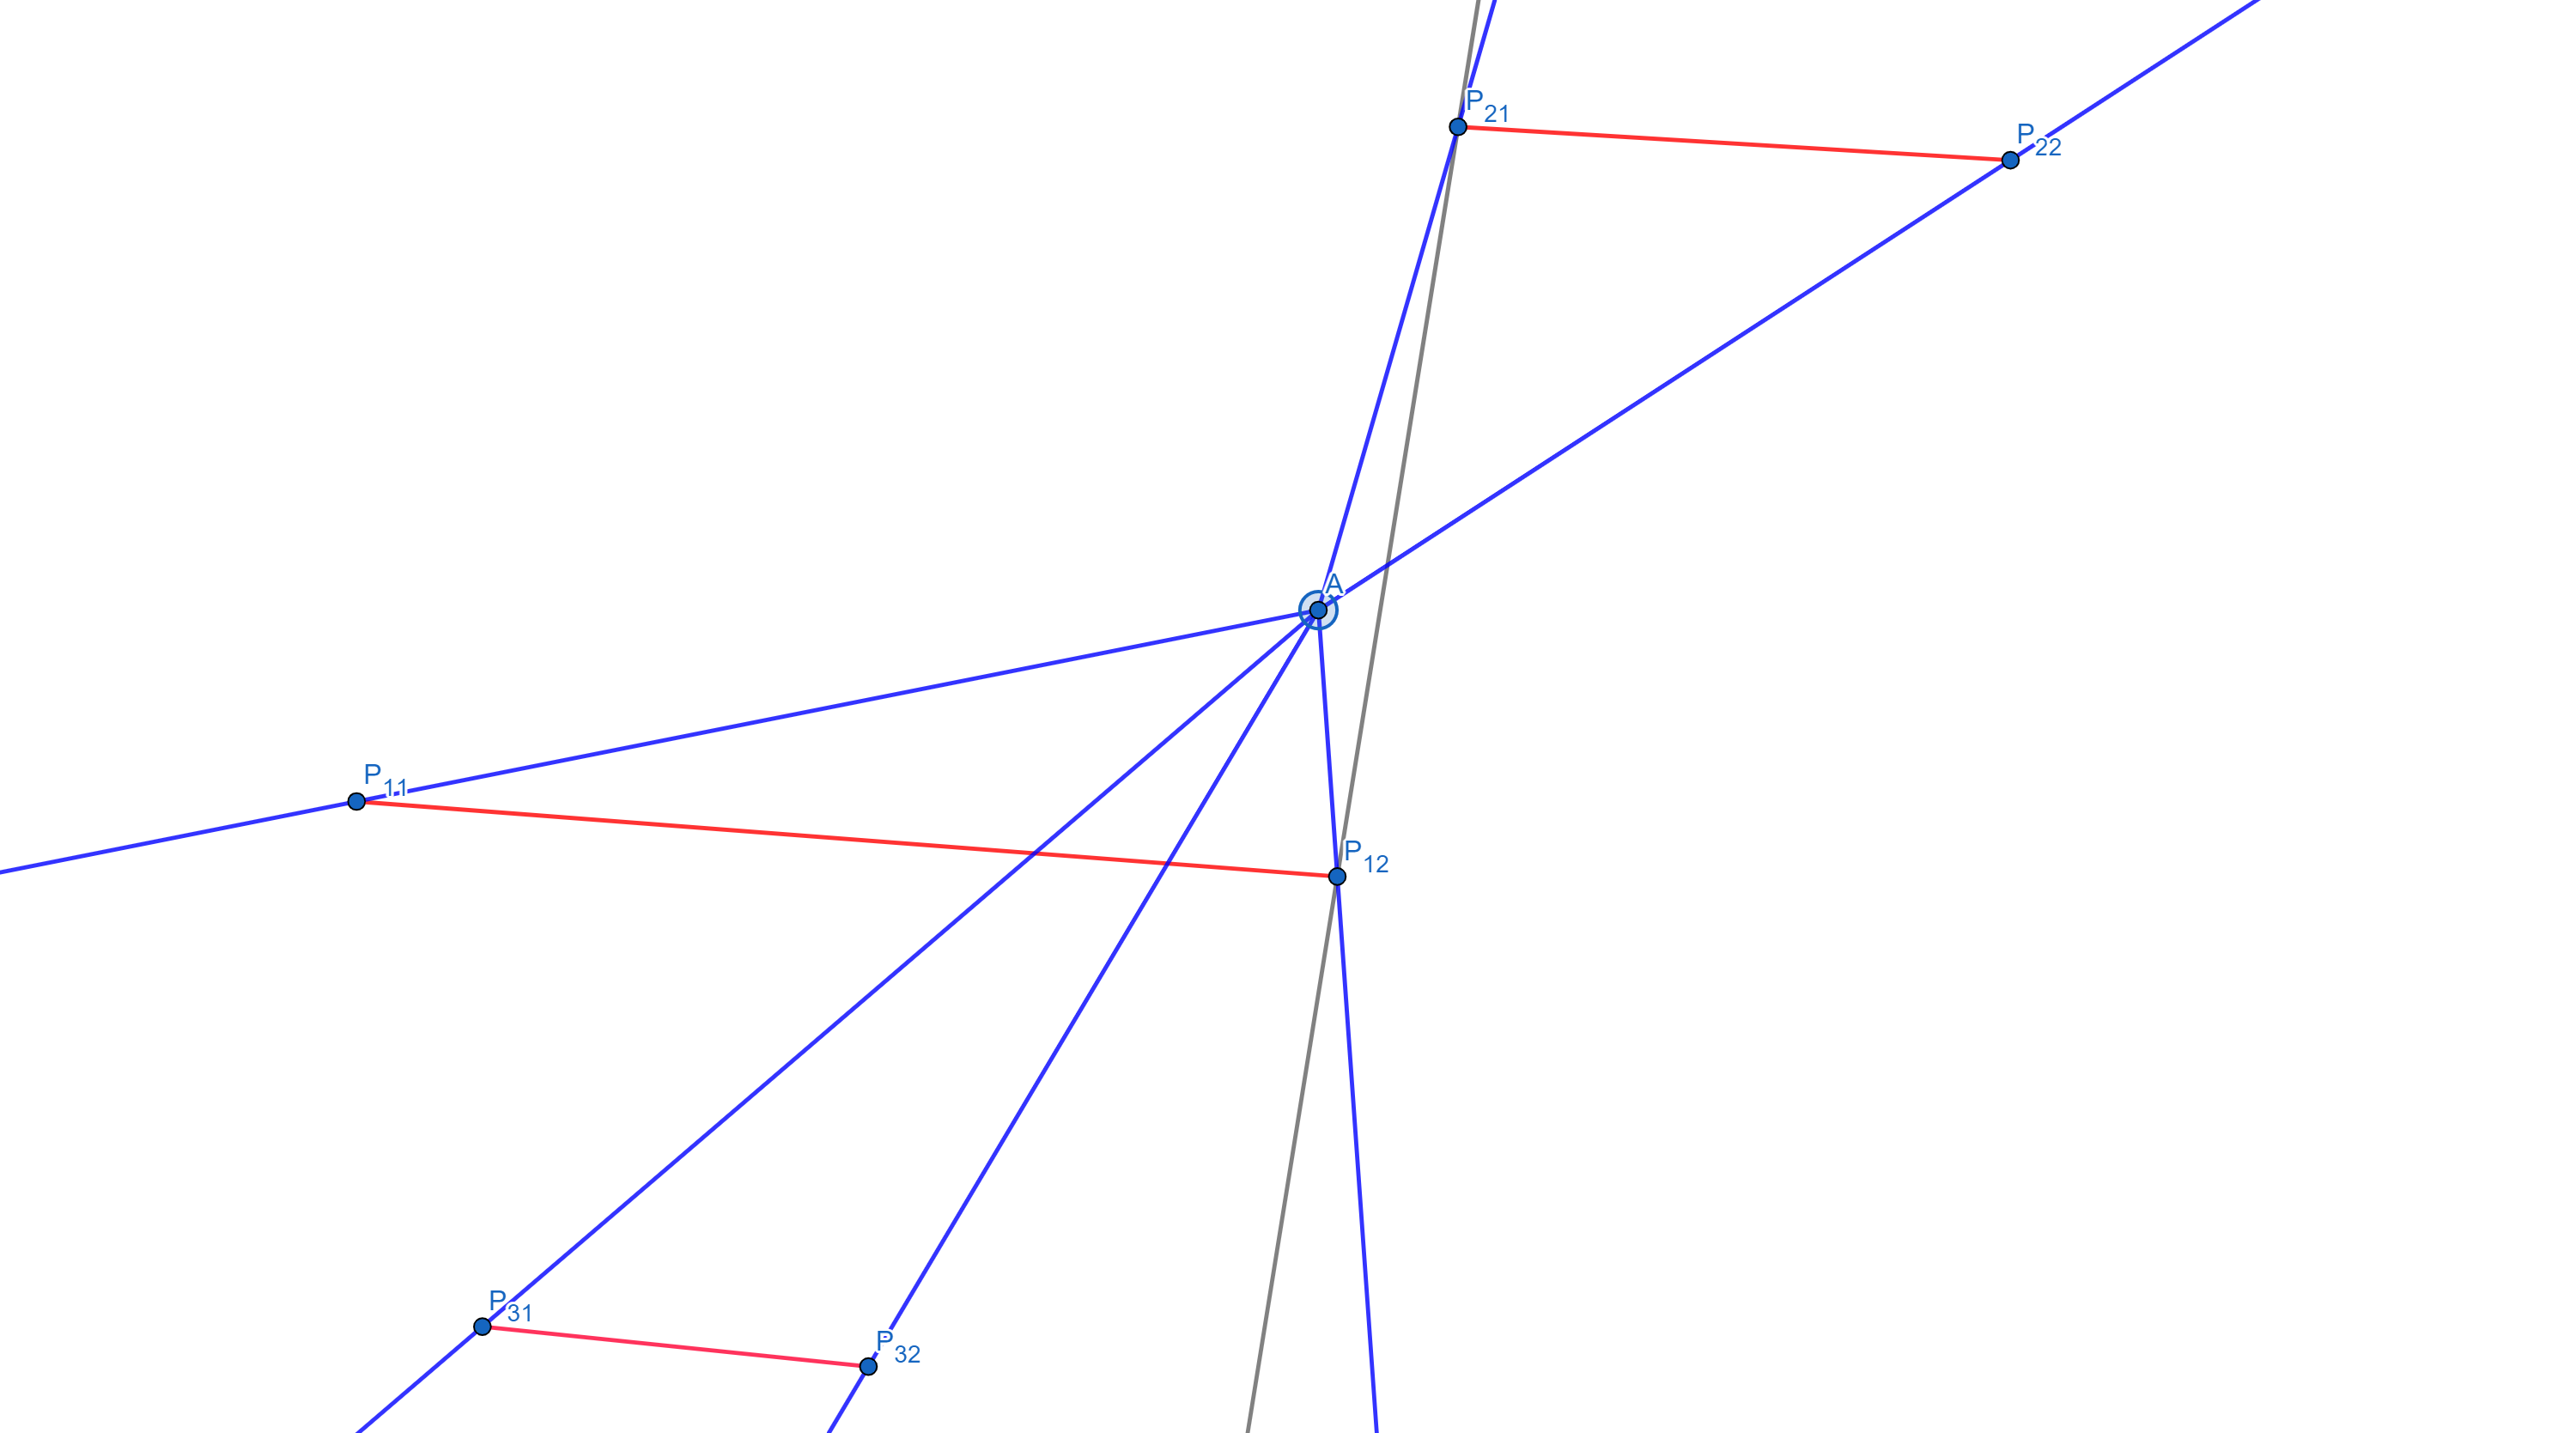
\includegraphics[width=0.5\linewidth]{between_1_1.png}
            \end{figure}
            \begin{figure}[H]
            \centering
            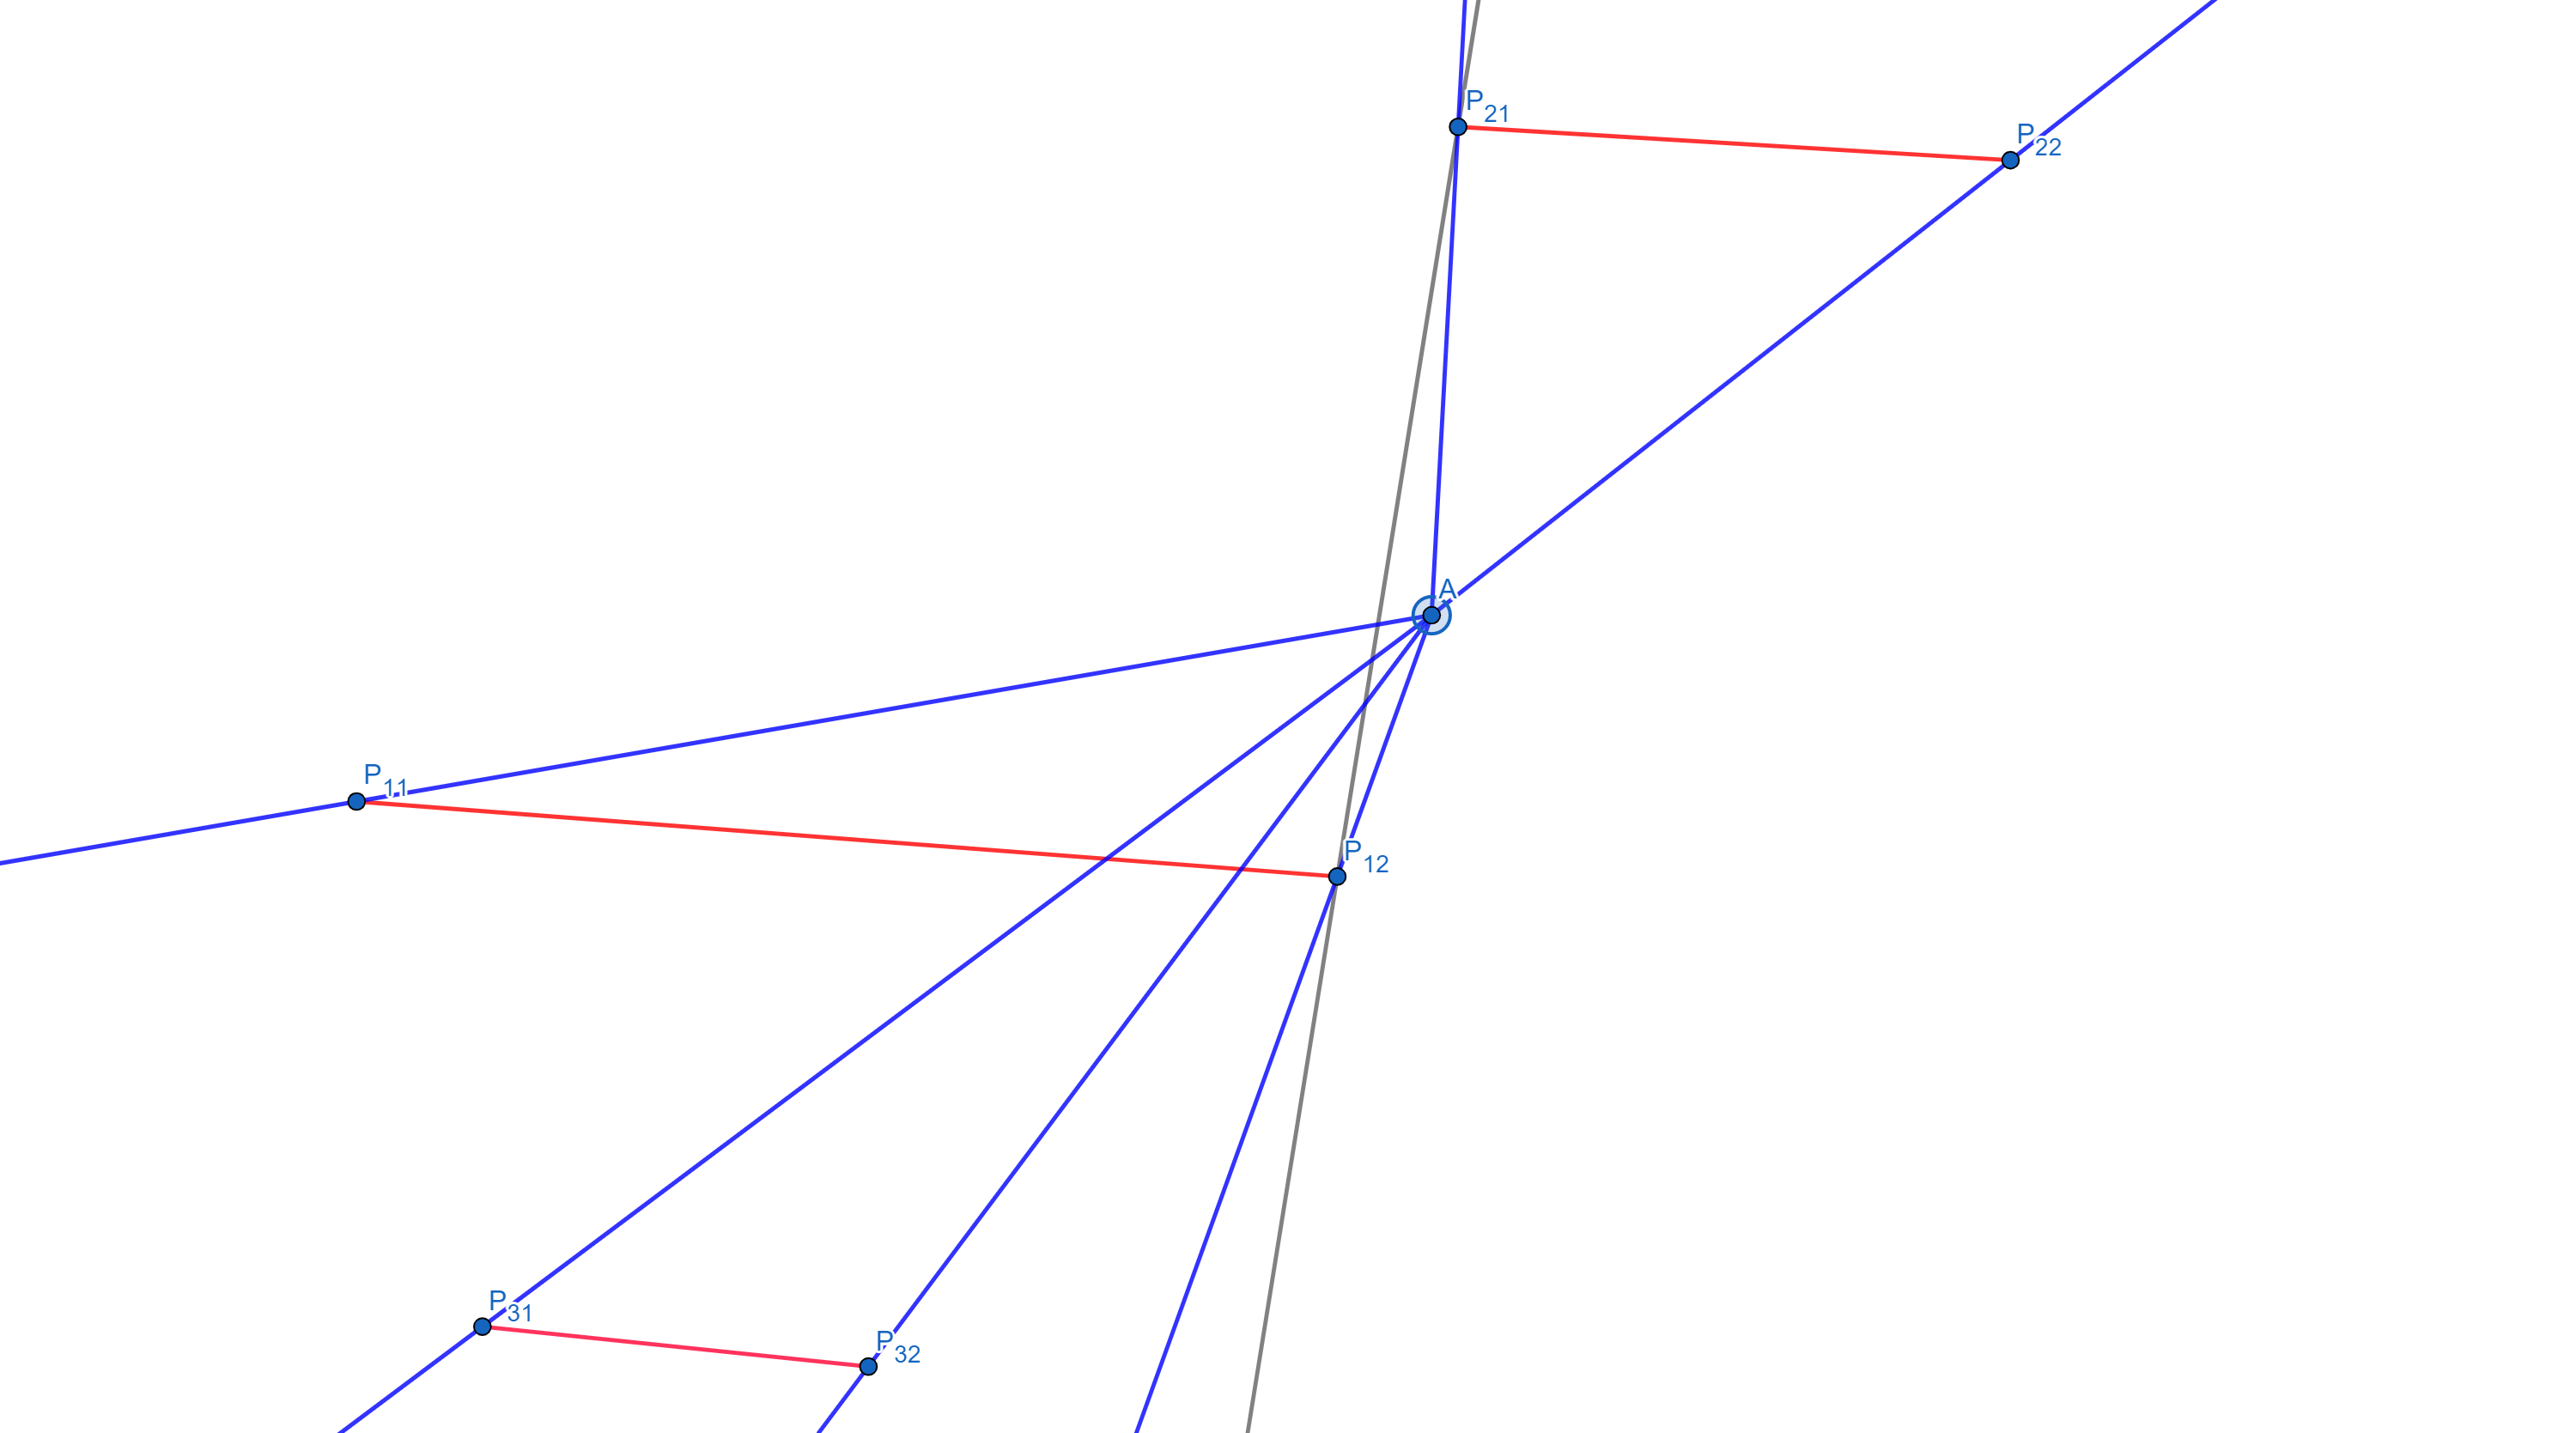
\includegraphics[width=0.5\linewidth]{between_1_2.png}
            \end{figure}
      \item Без изменений.
            \begin{figure}[H]
            \centering
            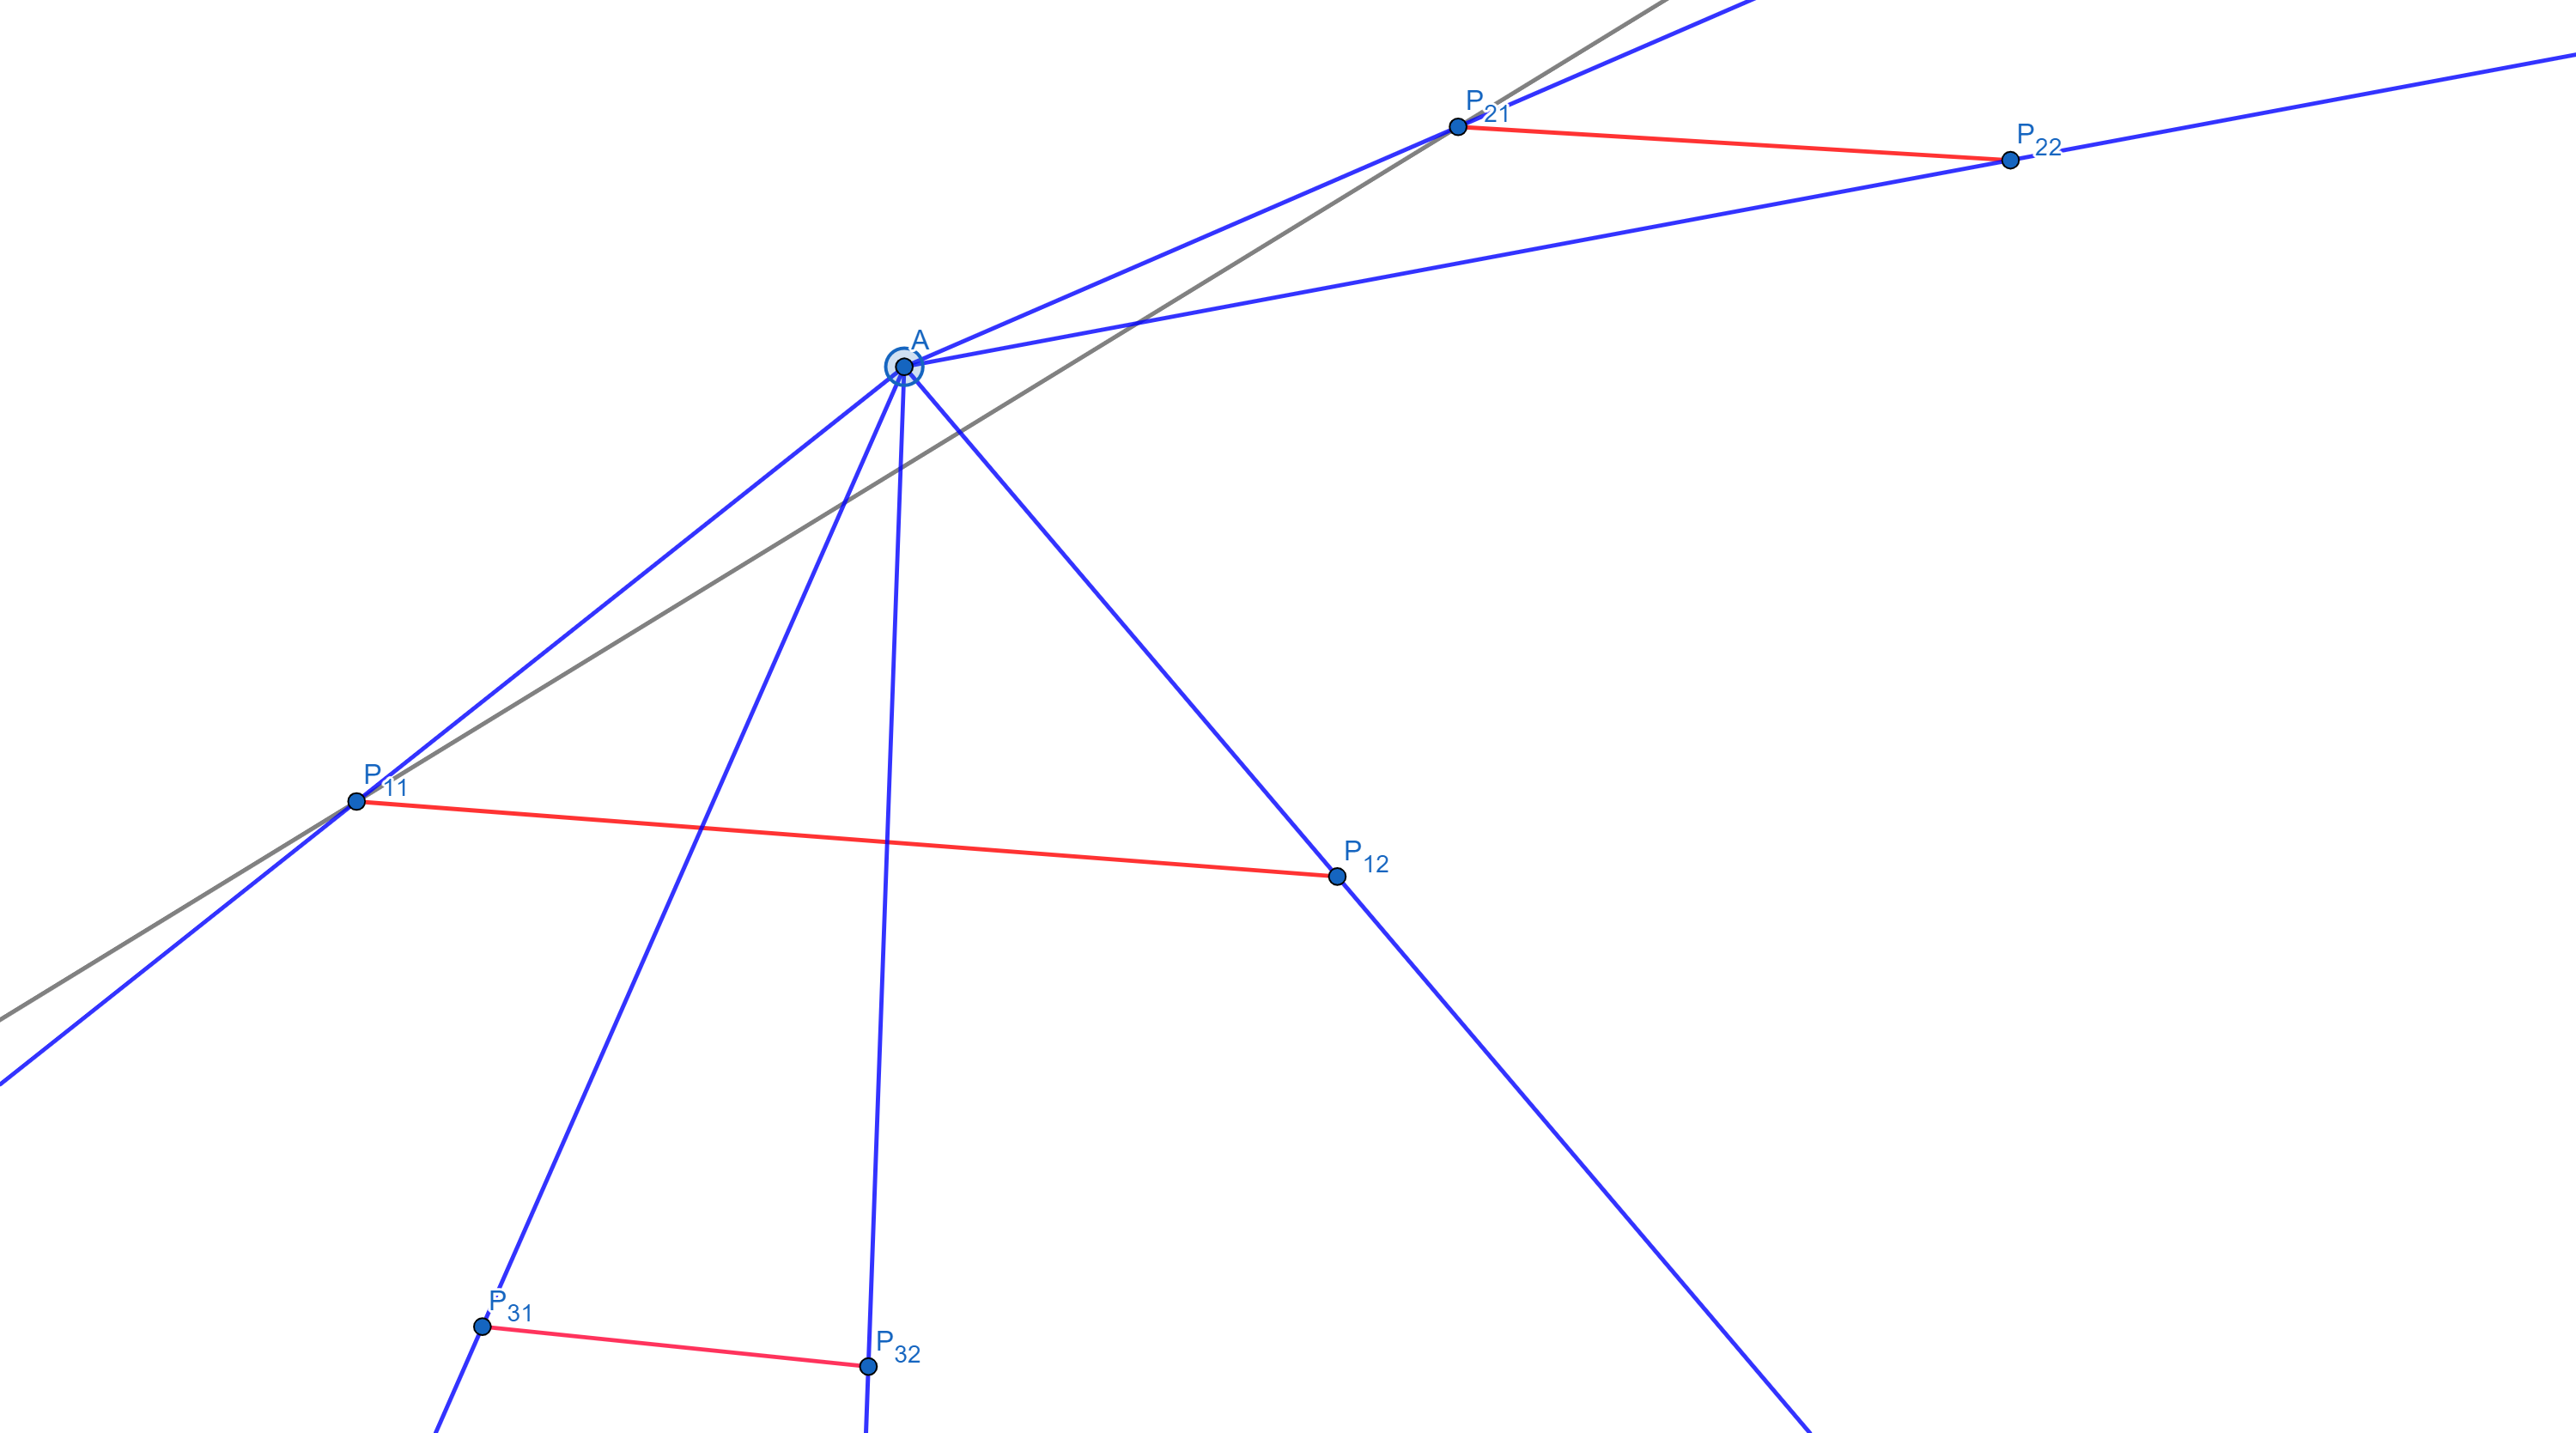
\includegraphics[width=0.5\linewidth]{between_2_1.png}
            \end{figure}
            \begin{figure}[H]
            \centering
            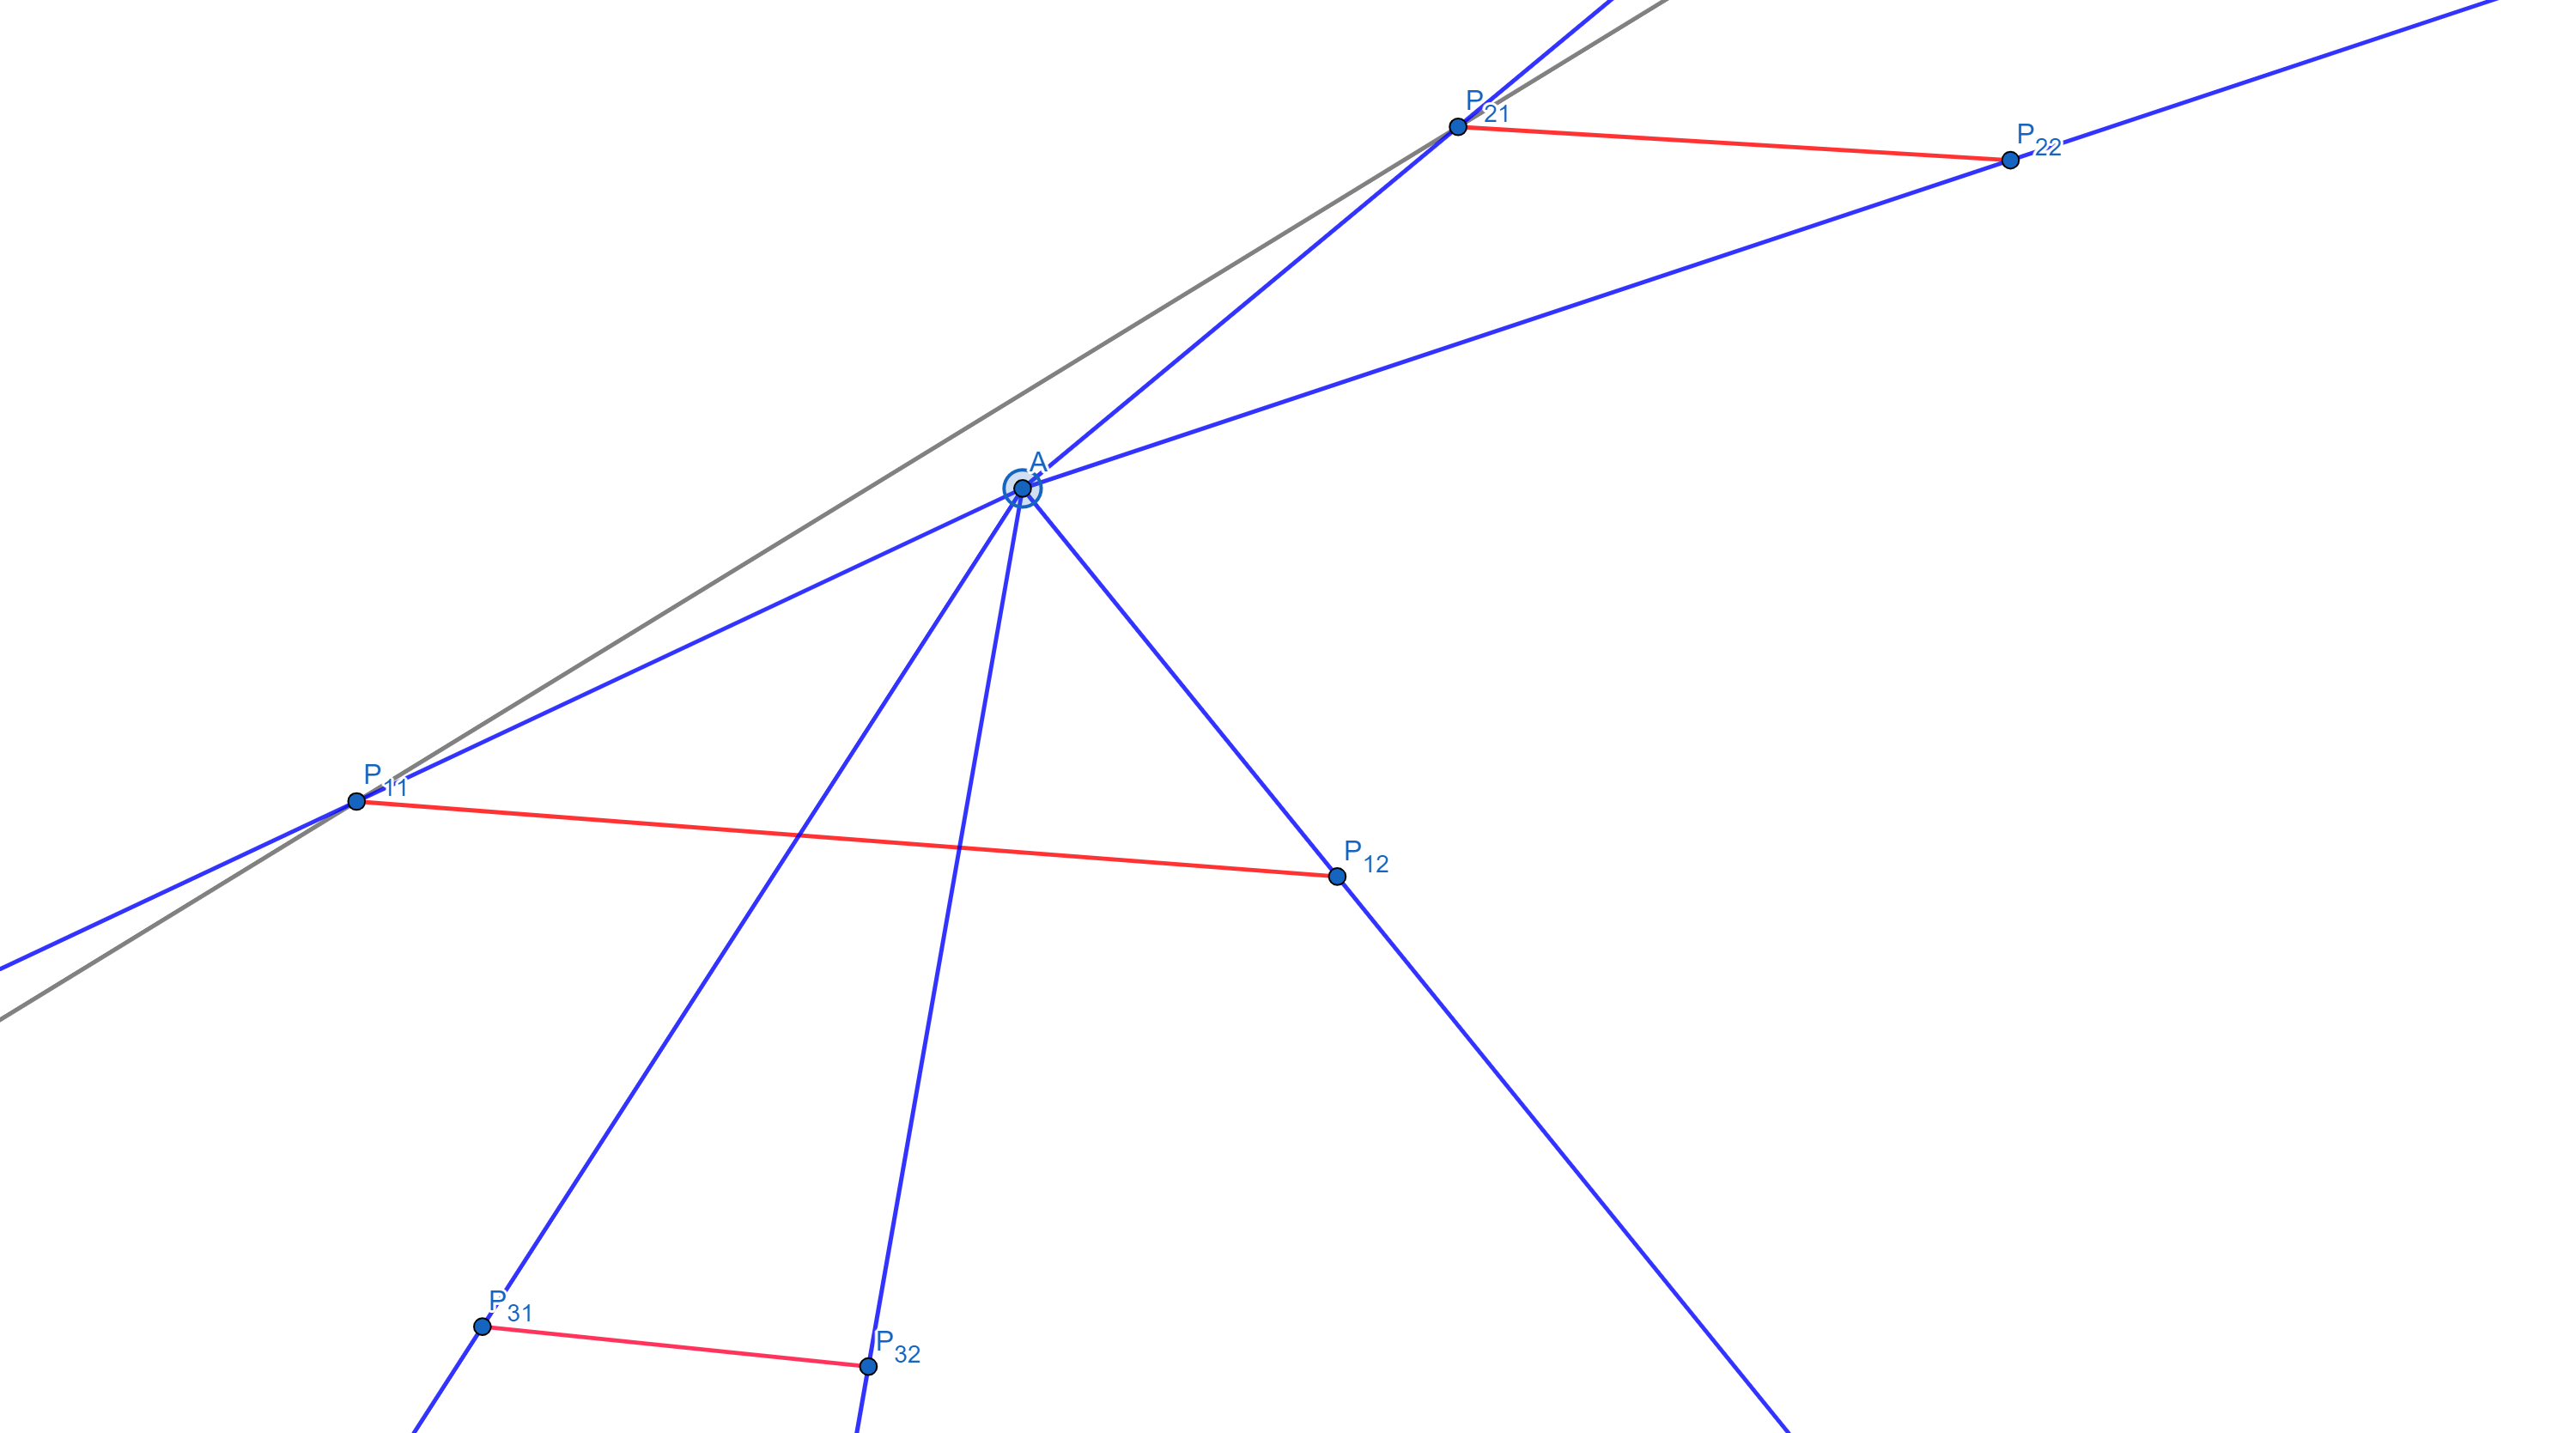
\includegraphics[width=0.5\linewidth]{between_2_2.png}
            \end{figure}
\end{enumerate}
\end{document}